\documentclass[10pt,landscape]{article}
\usepackage{amssymb,amsmath,amsthm,amsfonts}
\usepackage{multicol,multirow}
\usepackage{calc}
\usepackage{ifthen}
\usepackage{graphicx}
\usepackage{xcolor}
\usepackage[utf8]{inputenc}
\usepackage{enumitem} % For customizing lists
\usepackage{listings} 
\usepackage[landscape]{geometry}
\usepackage[colorlinks=true,citecolor=blue,linkcolor=blue]{hyperref}
\usepackage{fancyhdr}
\usepackage{tabularx}
\usepackage{lmodern}
\usepackage{soul} 
\usepackage{tikz}
\usepackage{colortbl}


% Global settings for itemize and enumerate
\setlist[itemize]{topsep=0pt, noitemsep, wide=0pt, leftmargin=\dimexpr\labelwidth + 2\labelsep\relax}
\setlist[enumerate]{topsep=0pt, noitemsep, wide=0pt, leftmargin=\dimexpr\labelwidth + 2\labelsep\relax}

\lstset{
    tabsize=2,    
%   rulecolor=,
    language={java},
        captionpos = t,
        basicstyle = \scriptsize\ttfamily,
        frame=lines,
        numbersep=5pt,
        numbers=left,
        numberstyle=\scriptsize,
        backgroundcolor=\color{white},
        columns=fixed,
        extendedchars=false,
        breaklines=true,
        prebreak = \raisebox{0ex}[0ex][0ex]{\ensuremath{\hookleftarrow}},
        frame=single,
        showtabs=false,
        showspaces=false,
        showstringspaces=false,
        keywordstyle=\color[rgb]{0,0,1},
        keywordstyle=[2]\color{gray},
        commentstyle=\color{teal},
        stringstyle=\color{red},
        numberstyle=\color[rgb]{0.205, 0.142, 0.73},
}

\ifthenelse{\lengthtest { \paperwidth = 11in}}
    { \geometry{top=.20in,left=.20in,right=.20in,bottom=.20in} }
	{\ifthenelse{ \lengthtest{ \paperwidth = 297mm}}
		{\geometry{top=1cm,left=1cm,right=1cm,bottom=1cm} }
		{\geometry{top=1cm,left=1cm,right=1cm,bottom=1cm} }
	}
\pagestyle{empty}
\makeatletter
\renewcommand{\section}{\@startsection{section}{1}{0mm}%
                                {-1ex plus -.5ex minus -.2ex}%
                                {0.5ex plus .2ex}%x
                                {\normalfont\large\bfseries}}
\renewcommand{\subsection}{\@startsection{subsection}{2}{0mm}%
                                {-1explus -.5ex minus -.2ex}%
                                {0.5ex plus .2ex}%
                                {\normalfont\normalsize\bfseries}}
\renewcommand{\subsubsection}{\@startsection{subsubsection}{3}{0mm}%
                                {-1ex plus -.5ex minus -.2ex}%
                                {1ex plus .2ex}%
                                {\normalfont\small\bfseries}}
\newcommand{\subsubsubsection}{\@startsection{subsubsection}{3}{0mm}%
                                {-1ex plus -.5ex minus -.2ex}%
                                {1ex plus .2ex}%
                                {\normalfont\scriptsize\bfseries}}
\newcommand{\Mod}[1]{\ (\mathrm{mod}\ #1)}
\makeatother
\setcounter{secnumdepth}{0}
\setlength{\parindent}{0pt}
\setlength{\parskip}{0pt plus 0.5ex}
\definecolor{mathblue}{cmyk}{1,.72,0,.38}
\everymath\expandafter{\the\everymath \color{mathblue}}

\renewcommand{\familydefault}{\sfdefault}
\renewcommand\rmdefault{\sfdefault}

\DeclareMathAlphabet{\mathmybb}{U}{bbold}{m}{n}
\newcommand{\1}{\mathmybb{1}}

\newenvironment{tightcenter}{%
  \setlength\topsep{0pt}
  \setlength\parskip{0pt}
  \begin{center}
    }{%
  \end{center}
}

\usepackage{soul}
\definecolor{paleyellow}{RGB}{251,243,218}
\newcommand{\definition}[2][]{\sethlcolor{paleyellow}\hl{\textbf{#2}} #1  $\rightarrow$}
% inline definition
\newcommand{\ildefinition}[1]{\sethlcolor{paleyellow}\hl{\textbf{#1}}}

\newenvironment{niceproof}[1][Proof]
{%
  \sbox0{\textit{#1}. }%
  \list{}{\labelwidth\wd0 \leftmargin\wd0 \labelsep 0pt }
\item[\usebox0]}
  {\endlist}

\title{CS4222-cheatsheet}
% -----------------------------------------------------------------------

\begin{document}

\raggedright
\scriptsize


\begin{multicols*}{3}
\setlength{\premulticols}{0.1pt}
\setlength{\postmulticols}{0.1pt}
\setlength{\multicolsep}{0.1pt}
\setlength{\columnsep}{0.1pt}
\begin{tiny}
    \small{\textbf{CS4222 Cheatsheet AY24/25 || \href{https://github.com/JasonYapzx}{@JasonYapzx}}} \\
\end{tiny}

% \subsubsubsection{Fundementals of electromagnetic waves}
\begin{itemize}
%     \item EM waves are synchronized oscillations of electric + magnetic field. There is a periodic change of eletric and magnetic fields.
%     \item How \textbf{often} this periodic change occurs dictates the property of EM waves
%     \begin{itemize}
%         \item Changer period is termed as the \textit{frequency}. SI unit is Hertz (Hz)
%         \item 1 Hz: 1 cycle of an electromagnetic wave in a second
%     \end{itemize}
    \item \textbf{Wavelength:} of sinusoidal waveform travelling at speed $v$, freq $f$ is $\lambda = \frac{v}{f}$
    \item EM waves travelling in free space, speed of light ($c \approx 3 \times 10^8$ m/s)
\end{itemize}

% \subsubsubsection{Radio Terminology}
% Implies the task of transmission and reception of information using EM waves of frequencies \textbf{3 Hz to 300 GHz}. EM Waves at these frequencies are also known as radio waves (frequency bands are also called the radio spectrum).
% \begin{itemize}
%   \item \textbf{Spectrum} To describe it as waves | EM Spectrum from smallest $\lambda$ to largest $\lambda$: Gamma $\rightarrow$ X-Ray $\rightarrow$ UV $\rightarrow$ Visible Light $\rightarrow$ Infrared $\rightarrow$ Microwave $\rightarrow$ Radio
%   \item \textbf{Characteristics:}
%   \begin{itemize}
%     \item Strength/Power: energy contained in the radio wave
%     \item Frequency: rate of periodic variation between electric/magnetic field
%     \item Bandwidth: range of frequencies of radio waves present in transmission
%     \item Polarization: orientation of electric field. (circular, elliptical, linear)
%     \item Modulation: variation of waves property to encode information
%   \end{itemize}
% \end{itemize}

% \subsubsubsection{How radio waves radiate out from transceiver}
% \begin{itemize}
%   \item \textbf{Antenna:} electical conductor/system of conductors:
%   \begin{itemize}
%     \item \textit{Transmission:} radio frequency electrical energy converted into electromagnetic energy | \textit{Reception:} reverse occurs, electromagnetic energy converted into electrical energy 
%     \item Antennas can be catogorized into directional/omnidirectional | based on radiation pattern of the antenna
%   \end{itemize}
% \end{itemize}

% \includegraphics*[width=8.5cm, height=2.8cm]{images/antennadirection.png}

% \subsubsubsection{Types of antennas}
% \begin{enumerate}
%   \item \textbf{Monopole:} straight ware mounted on conductive surface (ground plane)
%   \item \textbf{Array:} set of connected antenna elements working together
%   \item \textbf{Loop:} Loop or wire or conductor that acts like an antenna
%   \item \textbf{Aperture:} Transmits/receives EM waves through a hole
%   \item \textbf{Dipole:} Simple antenna consisting of wires pointed in opposite directions arranged horizontally/verically. End of each wire connected to radio and the other is hanging in free space.
%   \item \textbf{Half-wave Diploe:} More efficient variation of dipole, radiates energy efficiently when the wavelength of the radio signal is twice the electical length of antenna
% \end{enumerate}

\subsubsubsection{Relationship between antenna size and frequency}
Antenna size is \textbf{inversely proportional} to frequency of radio wave
\begin{itemize}
  \item Higher frequency, smaller antenna size, Lower frequency, larger size
  \item Dipole: length of conductor is $\frac{1}{2}$ of wavelength of radio wave
  \item Half-Dipole: length of conductor is $\frac{1}{4}$ of wavelength of radio wave
\end{itemize}

\subsubsubsection{Performance of an antenna}
\begin{itemize}
  \item \textbf{Gain of antenna:} Dimensionless ratio (unitless in linear form), commonly expressed in decibels (dB) or dBi. It measures the ability of an antenna to focus energy in a particular direction compared to a reference.
  \begin{itemize}
    \item \textbf{dBi}: Gain referenced to a theoretical isotropic antenna (uniform radiation in all directions)
    \item \textbf{dBd}: Gain referenced to a half-wave dipole antenna ($dBd = dBi - 2.15$)
  \end{itemize}
  \item \textbf{Units:}
  \begin{itemize}
    \item Linear gain ($G$) is unitless
    \item Logarithmic gain ($G_{\text{dB}}$ or $G_{\text{dBi}}$) is in decibels (dB)
    \item Convert: $G_{\text{dB}} = 10 \log_{10}(G_{\text{linear}})$ and $G_{\text{linear}} = 10^{G_{\text{dB}} / 10}$
  \end{itemize}
  \item \textbf{When to convert:}
  \begin{itemize}
    \item Use **linear gain** in physical formulas (e.g., Friis, $G = \frac{4 \pi A_e}{\lambda^2}$)
    \item Use **dBi/dB** when doing link budget calculations (additive terms with power in dBm, FSPL in dB, etc.)
  \end{itemize}
  \item $\uparrow$ gain $\Rightarrow$ more directional transmission/reception $\Rightarrow$ narrower beamwidth
\end{itemize}

\begin{multicols}{2}
  \[
    \boxed{G = \frac{4 \pi A_e}{\lambda^2} = \frac{4 \pi f^2 A_e}{c^2}}
  \]
  \columnbreak
  \begin{itemize}
    \item $G$ = antenna gain (unitless)
    \item $A_e$ = effective aperture area (m$^2$)
    \item $f$ = carrier frequency (Hz)
    \item $c$ = speed of light $3 \times 10^8$ m/s
    \item $\lambda$ = carrier wavelength (m)
  \end{itemize}
\end{multicols}

\begin{itemize}
  \item \textbf{Effective area:} Related to the physical size and shape of the antenna—larger $A_e$ typically yields higher gain.
  \item Power output evaluated in a direction, relative to isotropic antenna output.
  \item Relationship between gain and number of elements in an array: $G_{\text{array}} = G_{\text{single element}}(\text{dBi}) + 10 \log_{10}(N)$, where $N$ is the number of antenna elements; $10 \log_{10}(N)$ is the array factor.
\end{itemize}

% \subsubsubsection{How do radio waves propagate from TX to RX}
% Radio wave propagation is heavily influenced by the medium and environment (e.g., poor underwater). Environmental factors like obstacles, interference, and weather significantly impact communication range and reliability
% \begin{itemize}
%     \item \textbf{Line-of-Sight (LoS):} Requires a clear path between antennas. Used in satellite comms ($>30$ MHz signals aren't reflected by ionosphere) and ground comms (effective LoS aided by refraction)
%     \item \textbf{Non-Line-of-Sight (NLoS):} Scenario where signals encounter obstacles (walls, buildings), reflect, take multiple paths, and are affected by weather
% \end{itemize}

% \subsubsubsection{How do radio waves propagate from TX to RX}
% \begin{itemize}
%   \item Medium and enviornment has an important role to play in propagation
%   \item Radio waves do not propagate well underwater. Submarines uses sound
%   \item Environment impacts the radio wave propagation significantly
%   \begin{itemize}
%     \item Reduced communication range
%     \item Interference from other devices
%     \item Issues with reliability
%   \end{itemize}
% \end{itemize}

% \subsubsubsection{Radio waves propagation in line-of-sight}
% \begin{itemize}
%   \item Transmitting and receiving antennas must be within line of sight (nothing interfering with communication)
%   \item Satellite communication | signal above 30 MHz not reflected by ionosphere
%   \item Ground communication | antennas in effective line of site due to refraction
% \end{itemize}

% \subsubsubsection{Non Line-of-sight}
% \begin{itemize}
%   \item But real-world is not so simple, as it can be bounced off surfaces, has multiple paths or even be affected by weather
%   \item Transmitter and receiver are not kept in line of sight
%   \item Radio waves encounter obstacles, may go through walls, buildings
%   \item Much more applicable to read world environment and deployments
%   \item Significantly impacts the communication range/reliability
% \end{itemize}

% \subsubsubsection{Radiation pattern of antenna}
% \begin{itemize}
%   \item graphical representation of relative strength of radiated power in various directions $\rightarrow$ illustrates how antenna distributes energe in space
%   \item radiation pattern is represented as a polar/rectangular plot
%   \item helps to understand the nature of antenna: isotropic, directional, or omnidirectional $\rightarrow$ helps optimize the placement of wireless devices
% \end{itemize}

% \includegraphics*[width=8.5cm, height=2.8cm]{images/radiationpattern.png}

% \subsubsubsection{Understanding the antenna beamwidth}
% \begin{itemize}
%   \item Antenna beamwidth is the angular separation between the points on the radiation pattern where the power drops to $\frac{1}{2}$ its max value
%   \item Main lobe of radiation pattern where \underline{max radiation occurs} | Commonly known as the $-3$ dB points. Defines the directivity/coverage area of antenna
% \end{itemize}

\subsubsubsection{Choosing Beamwidth: Tradeoffs}
\begin{itemize}
    \item \textbf{Narrow beamwidth}: Offers higher directivity and longer range due to increased gain, making it suitable for point-to-point links.
    \item \textbf{Broader beamwidth}: Covers a larger area but has lower directivity and range due to lesser gain, making it suitable for broadcast applications.
\end{itemize}

\subsubsubsection{Attenuation and Gain: Decibel (dB) unit}
\begin{itemize}
  \item \textbf{Attenuation:} Loss of energy when signal traverses through a medium
  \item \textbf{Gain:} $\uparrow$ in energy $\rightarrow$ devices employed to improve signal strength
  % \item Commonly we use decibel to calculate gain/loss or attenuation of signal
  \item \framebox{$dB = 10\log_{10} \frac{P_2}{P_1}$} (where $P_1$ is input power, $P_2$ is output power)
  \item e.g. supposed signal travels through transmission medium, power $\downarrow$ to $\frac{1}{2}$ original value, meaning $P2 = \frac{1}{2} P1$.
  \item $10\log_{10}\frac{P_2}{P_1} = 10\log_{10}\frac{0.5P_1}{P_1} = 10\log_{10}0.5 = 10(-0.3) = -3dB$
  \item Effectively, loss of $3dB$ is equivalent fo losing half of the signal power
\end{itemize}

\subsubsubsection{Unit of power of a signal: dBm (decibel milliwatt)}
\begin{itemize}
  \item Decibel (dBm) is a measure of signal power, calculated as $10\log 10(P_m)$ where $P_m$ is power in milliwatts ($mW$)
  \item $0 \ dBm$ represents a transmit power of $1 mW \rightarrow$ common reference point in communication systems
  \item $30 \ dBm$ which corresponds to transmit power of $1 W$ is often the maximum permissible output power for devices operating in unlicensed frequency bands, e.g. those in Wi-Fi and other wireless communication technologies.
\end{itemize}

\subsubsubsection{Estimating received signal strength and range: Friis propagation model}
\begin{multicols}{2}
  \begin{center}
    \[
      \boxed{P_r = G_r G_t \left(\frac{c}{4\pi f_c d}\right)^a P_t} 
    \]
    \tiny{(in \ dBm)}
  \end{center}

  \columnbreak
  \begin{itemize}
    \item $f_c$ center frequency in Hertz
    \item $c$ = speed of light
    \item $d$ = distance btw transmitter/receiver
    \item $a$ = path loss component
    \item $G$ = antenna gain
  \end{itemize}
\end{multicols}

{ 
\tiny
\begin{tabularx}{\columnwidth}{|X|X|}
  \hline
  \rowcolor{lightgray}
  \textbf{Environment} & \textbf{Path Loss Exponential ($\alpha$)} \\ \hline
  Free Space & 2 \\ \hline
  Urban area cellular radio & 2.7 to 3.5 \\ \hline
  Shadowed urban cellular radio & 3 to 5 \\ \hline
  In building LOS & 1.6 to 1.8 \\ \hline
  Obstructed in building & 4 to 6 \\ \hline
  Obstructed in factory & 2 to 3 \\ \hline
\end{tabularx}
}

\subsubsubsection{Free Space Path Loss | $FPSL (\text{linear}) = {\frac{4\pi d f }{c}}^2$}
\begin{itemize}
  \item Loss of power by signal as it transmits from the transmitter to receiver 
  \item $d$ is the distance between the transmitter and receiver antennas (in meters),
  \item $f$ is the frequency of signal (in Hertz), $c$ is speed of light in a vacuum
  \item \framebox{\parbox{\dimexpr\linewidth-1\fboxsep-150\fboxrule}{% 
  $FPSL = 20\log_{10}(d) + 20\log_{10}(f)+ 20\log_{10}(\frac{4\pi}{c})$
  }} \tiny{| in $dB$ always}
\end{itemize}

\subsubsubsection{Total link gain in wireless communication}
\begin{itemize}
  \item net amplification/attenuation of EM signal along the communication path
  \begin{itemize}
    \item Antennas, FSPL, any other system component is also included:
      \framebox{\parbox{\dimexpr\linewidth-1\fboxsep-150\fboxrule}{% 
        $\text{(dB)} = G_{Tx} + G_{Rx} - L_{Path} - L_{Misc}$
      }}
      \item $G_{Tx}$ = Transmitter antenna gain (dB)
      \item $G_{Rx}$ = Receiver antenna gain (dB)
      \item $L_{Path}$ = Path loss (dB), including free-space loss
      \item $L_{Misc}$ = misc losses (dB), (atmospheric/cable losses/interference)
  \end{itemize}
\end{itemize}

\subsubsubsection{Link Budget and Total Link Gain}
\begin{itemize}
  \item Calculation that takes into account all gains/losses to determine received signal strength of wireless signal in a communication system
  \item Total Link Budget ($P_{rx}$) = $P_{tx} + $ Total Link Gain 
  \item \textbf{Total Link Budget} \framebox{\parbox{\dimexpr\linewidth-1\fboxsep-280\fboxrule}{% 
    $ P_{Rx}= P_{Tx} + G_{Tx} + G_{Rx} - L_{Total}$
  }}
  \begin{itemize}
    \item $P_{\text{Tx}}$ = Transmit power in dBm.
    \item $G_{\text{Tx}}$ = Transmit antenna gain in dBi.
    \item $G_{\text{Rx}}$ = Receive antenna gain in dBi.
    \item $L_{\text{Total}}$ = Total losses (e.g., free space path loss, cable losses) in dB.
    \item $P_{\text{Rx}}$ = Received power in dBm.
  \end{itemize}
\end{itemize}

\subsubsubsection{dB, dBm and dBi operations}
\begin{itemize}
  \item db (Decibel): log unit for ratios (gain/loss), dimensionless
  \item dBm: absolute power reference to $1mW$, $0 dBm = 1mW$
  \item dBi: Antenna gain relative to isotropic radiator. Measures directionality
  \item \textbf{Adding dB values:}
  \begin{itemize}
    \item If 2 components contribute gain/loss, we add their dB values
    \item e.g. 2 amplifiers with +10dB and +5dB gain
  \end{itemize}
  \item \textbf{Adding dBi to dBm to get EIRP}
  \begin{itemize}
    \item Effective Isotropic Radiated Power (EIRP): total output power including antenna gain: $EIRP = P_{TX}(dBm) + G_{antenna}(dBi)$
  \end{itemize}
  \item \textbf{Subtracting Losses (dB) from Power (dBm)}
  \begin{itemize}
    \item Losses (cable/FPSL) can be subtracted from transmitted power
  \end{itemize}
  \item \textbf{Subtracting dBm values to get dB diff.:} Used to compare 2 power EIRP
  \item \underline{You cannot add dBm values directly} as dBm represents absolute power, log values cannot be added directly
  \begin{itemize}
    \item Must convert to linear scale e.g. $10 dBm = 10mW + 20 dBm = 100 mW$, Total power = $110 mW = 10\log_{10}(110) = 20.4 dBm$
  \end{itemize}
\end{itemize}

\subsubsubsection{Operations with dB, dBm, and dBi}
{
\tiny 
\begin{tabularx}{\columnwidth}{|c|c|X|}
\hline
\rowcolor{lightgray}\textbf{Operation} & \textbf{Valid?} & \textbf{Explanation} \\
\hline
dBm + dBm & $\times$ & Log scale absolute powers can't be added directly \\
\hline
dBm + dBi & $\checkmark$ & EIRP calculation: antenna gain added to transmit power \\
\hline
dBm - dB & $\checkmark$ & Used to subtract path/cable losses \\
\hline
dB + dB & $\checkmark$ & Gains/losses (ratios) are additive in log scale \\
\hline
dBm to linear (mW) & $\checkmark$ & $P_{mW} = 10^{P_{dBm}/10}$ \\
\hline
Linear (mW) to dBm & $\checkmark$ & $P_{dBm} = 10 \log_{10}(P_{mW})$ \\
\hline
dBm + dBm (via linear) & $\checkmark$ & Convert to mW, sum, then log: $P_{total} = 10 \log_{10}(P_1 + P_2)$ \\ % Removed \newline
\hline
\end{tabularx}
}

% \subsubsubsection{How are radio waves modified to carry information}
% \begin{itemize}
%   \item Encoding information `basedband' in an analog `carrier' signal
%   \begin{itemize}
%     \item Baseband signal often much lower in frequence than carrier
%     \item Frequency of the carrier signal dictates the part of the radio spectrum
%   \end{itemize}
%   \item Why? baseband signals or info change at a much lower rate
%   \begin{itemize}
%     \item Speech up to $20KHz$, temp changes $\approx$ few $Hz$
%     \item Enables a better usage of the radio spectrum
%     \item Enables communication among several devices sharing the spectrum
%   \end{itemize}
%   \item Modulation techniques
%   \begin{itemize}
%     \item Vary frequency, amplitute, phase of carrier signal according to msg signal
%     \item OR vary them together to support complex modulation schemes
%     \item Analog / Digital counterparts of these modulations schemes exists
%   \end{itemize}
% \end{itemize}

\subsubsubsection{Modulation}
% \includegraphics*[width=8.5cm, height=1.7cm]{images/modulation.png}

\subsubsubsection{Amplitute modulation}
\begin{itemize}
  \item Change amplitute of carrier signal according to the message signal
  % \item Simplest and earliest modulation technical
  % \item Remains widely used for radio broadcast/computer communication
      \[
        \boxed{s(t) = [A_c + A_m \cdot m(t)] \cdot (2\pi f_c t)}
      \]
      \begin{multicols}{2}
        \begin{itemize} 
          \item $A_c$ Carrier Amplitute
          \item $A_m$ Baseband signal amplitude
          \item $m(t)$ Message signal
          \item $f_c$ Carrier Frequency
        \end{itemize}
    \end{multicols}
  \item \textbf{Modulation Index}
  \begin{itemize}
    % \item Signifies extent to which carrier signal modulated with message signal. Determines strength of modulated signal, impacts bandwidth and also power distribution and overall signal quality.
    \item For amplitude modulation $\mu (modulation \ index) = A_m / A_c$
    \begin{itemize}
      \item $A_m$ = Peak amplitude of modulating/baseband signal
      \item $A_c$ = Peak amplitude of carrier signal
      \item $\mu < 1$: under-modulated (weak signal, no distortion); $\mu = 1$: fully modulated; $\mu > 1$: over-modulated (distortion, clipping)
    \end{itemize}
  \end{itemize}
\end{itemize}

\subsubsubsection{Frequency modulation}
\begin{itemize}
  \item Change frequency of carrier signal according to the message signal
  \item Advantages over AM: resilient to interference, spectrum efficiency
  \item Remains widely used for radio broadcast, also computer communication
  \item Bandwidth of frequency modulated signals
      \[
        \boxed{s(t) = A_c cos (2\pi f_c t + 2\pi k_f \int m(t) dt))}
      \] 
    \begin{itemize}
      \item $A_c$ Carrier Amplitute, $f_c$ Carrier Frequency
      \item $k_f$ Frequency sensitivity of modulator (how much carrier freq. changes in response to amplitude of modulating signal)
      \item $m(t)$ Modulating signal
    \end{itemize}
  \item \textbf{Modulation Index}
  \begin{itemize}
    \item $\beta(modulation \ index) = \triangle f / fm$
    \item Given by Carson's rule, bandwidth is $2 (\triangle f + fm)$
    \item $\triangle f$ = Peak frequency deviation (how much carrier frequency changes)
    \item $f_m$ = Maximum frequency of the modulating signal
    \item $B < 1$: Narrow band signal, $B > 1$ Wideband signal, better noise immunity, signal quality, FM broadcast
  \end{itemize}
\end{itemize}

\subsubsubsection{What is a phase}
\begin{itemize}
  \item Represents position of point on waveform cycle, an offset from starting position of sine wave
  \item Complete cycle of sine wave is 360 degress / 2 $\pi$ radian
  \begin{multicols}{2}
      \[
        \boxed{s(t) = A \cos(2\pi ft + \phi)}
      \]
    \columnbreak
    \begin{itemize}
      \item $A$ = Amplitude of signal
      \item $f$ = Frequency of signal
      \item $\phi$ Phase (phase contstant / offset)
    \end{itemize}
  \end{multicols}
  \item $\phi$ determines where in its cyclewave is (begins at $t=0$)
  \item Changing $phi$ shifts waveform left or right in time
  \item \textbf{\underline{Impact of phase shifts on waves (summation)}} (interference)
  \begin{itemize}
    \item \textit{Constructive:} 2 waves with same phase add tgt to form larger amplitude
    \item \textit{Destructive:} 2 waves out-of-phase (e.g. 180$\deg$ apart), cancel each other
  \end{itemize}
\end{itemize}

\subsubsubsection{Phase modulation}
\begin{itemize}
  \item Change phase of carrier signal according to the message signal
  \item Integral part of modern communcation standards: Wifi/Television
  \item Advantages over FM: Better SNR and spectral efficiency
  \item Uses different phase shifts to represent digital data
  \begin{multicols}{2}
    \begin{center}
      \[
        \boxed{s(t) = A \cos(2\pi f_c t + 2\pi k_p m(t))}
      \]
    \end{center}
    \columnbreak
    \begin{itemize}
      \item $A$ = Amplitude of signal
      \item $f_c$ = Carrier frequency
      \item $k_p$ = Phase sensitivity (rad / unit amplitude)
      \item $m(t)$ = modulating signal
    \end{itemize}
  \end{multicols}
\end{itemize}

\subsubsubsection{Binary Phase Shift Keying}
\begin{itemize}
  \item simple form of phase modulation where phase is shifted between 2 values 
  \item \textit{Bit 0} $\rightarrow$ 0 degrees ($A\sin (2\pi f_c t)$)
  \item \textit{Bit 1} $\rightarrow$ 180 degrees ($A\sin(2\pi f_c t + \pi)$)
\end{itemize}
\includegraphics*[width=8.5cm, height=2.8cm]{images/bpsk.png}

\subsubsubsection{Quadrature Binary Phase Shift Keying}
\begin{itemize}
  \item extends BPSK with 4 distinct phase states, allow encoding of 2 bits/symbols
  \item \textit{Bit 00} $\rightarrow$ 45 degrees ($A\sin (2\pi f_c t + \pi/8)$)
  \item \textit{Bit 01} $\rightarrow$ 90 degrees ($A\sin(2\pi f_c t + \pi/4)$)
  \item \textit{Bit 10} $\rightarrow$ 135 degrees, \textit{Bit 11} $\rightarrow$ 225 degrees
  \item We are \textit{doubling the bit rate} for the same bandwidth
\end{itemize}

\subsubsubsection{Digital equivalent of AM FM and PM modulation}
\begin{itemize}
  \item Vary analog signal according to digital bits
  \begin{itemize}
    \item ASK: amplitute/FSK: frequency/PSK: phase shift keying
  \end{itemize}
  \item Digital variants relevant when we talk about computer communication
\end{itemize}

% \subsubsubsection{Wireless Link quality and Reliability}
% \begin{itemize}
%   \item Link reliability metrics quantify quality and stability of wireless links
%   \item Wireless links are unstable due to interference, multipath fading, mobility
%   \begin{itemize}
%     \item Helps in routing decisions optimizing network performance and improving communication reliability among other uses
%     \item From application perspective, no buffering and low latency
%   \end{itemize}
% \end{itemize}

\subsubsubsection{Link Quality Metrics:}
\begin{itemize}
  \item \textbf{Packet Delivery Ratio (PDR)}: ratio of successfully received packets to transmitted packets. \framebox{\parbox{\dimexpr\linewidth-1\fboxsep-280\fboxrule}{% 
    $PDR = \frac{Received \ Packets}{Transmitted \ Packets} \times 100$
  }}
  \begin{itemize}
    \item $\uparrow$ = better link quality, $\downarrow$ = congestion/interference or poor connectivity
  \end{itemize}
  \item \textbf{Bit Error Rate (BER):} Ratio of bits received in error to the total transmitted bits. Indicates transmission quality at the physical layer
  \begin{itemize}
    \item \framebox{\parbox{\dimexpr\linewidth-1\fboxsep-240\fboxrule}{% 
      $BER = \frac{Errored \ Bits}{Total \ Bits \ Transmitted} \times 100$
    }}
    \item $\downarrow$ = fewer errors + better link perf. $\uparrow$ = data corruption / retransmissions
    \item Wired Ethernet: $10^{-12}$, Wireless Wifi: $10^{-6}$ to $10^{-3}$, Poor cxn = $10^{-2}$ 
  \end{itemize}
  \item \textbf{Signal-to-Noise Ratio (SNR):} Ratio of signal power to background noise, often measured in decibels. \framebox{\parbox{\dimexpr\linewidth-1\fboxsep-250\fboxrule}{% 
    $SNR = 10\log_{10}(\frac{P_{signal}}{P_{noise}})$ | if $P$ in $W$
  }}
  \begin{itemize}
    \item Else $P_{signal} - P_{noise}$ in $dBm$
    \item $\uparrow$ = stronger signal, fewer errors. $\downarrow$ = more packet loss. 
  \end{itemize}
  \item \textbf{Expected Transmission Count (ETX):} Measures expected number of trasmissions (including re-trasmission) required for packet to successfully received. Used in routing algorithms \framebox{\parbox{\dimexpr\linewidth-1\fboxsep-340\fboxrule}{% 
    $ETX = \frac{1}{P_{forward} \times P_{reverse}}$
  }} 
  \begin{itemize}
    \item Lower ETX means fewer transmission and better efficiency, higher leads to increased latency and power consumption
  \end{itemize}             
\end{itemize}

\subsubsubsection{Understanding Channel Capacity \& Link Quality}
\begin{itemize}
    \item \textbf{Definition:} Maximum rate at which information can be transmitted over a communication channel without error.
    \item Channel capacity is measured in the unit of \textbf{bits/second}.
    \item How does channel capacity relate to link quality?
    \begin{itemize}
        \item Higher \textbf{SNR} usually leads to a higher capacity.
        \item Recall bandwidth is the frequency range over which the signal is transmitted; a wider bandwidth can support higher data rates.
        \item Factors that reduce link quality: \textbf{Fading, interference}, reducing channel capacity.
    \end{itemize}
    \item Channel Capacity and Link Quality | Shannon Perspective:
    \begin{multicols}{2}
      \begin{center}
        \[
          C = B \times \log_2(1 + \frac{S}{N})
        \]
      \end{center}
      \columnbreak
      \begin{itemize}
        \item $C$ Channel capacity in bits per second (bps)
        \item $B$ = Bandwidth of the channel in Hertz (Hz)
        \item $S/N$ Signal-to-noise ratio (SNR) expressed as linear ratio
      \end{itemize}
    \end{multicols}
\end{itemize}

\subsubsubsection{Processors, Memory, Contiki}
\begin{itemize}
  \item Microcontroller ($\mu C$) small computer on single integrated circuit on simple CPU with peripheral devices (I/O, timers, memories)
  \item Low power, often include sleep mode that dramatically reduces the power consumed to micro or even nanowatts
\end{itemize}

\subsubsubsection{ISA and Realization}
\begin{itemize}
  \item \textbf{Instruction set architecture:} definition of instructions that processor can execute and certain structural constraints (such as word size) that realizations must share
  \item \textbf{Processor, Realization Chip:} Piece of silicon sold by vendor which is realization of the ISA
  \item A ISA may appear in many different chips often made by different manufacturers with widely varying performance profiles
\end{itemize}

\subsubsubsection{Digital Signal Processor}
\begin{itemize}
  \item Deal with large amounts of information, Sample in time/space/both
  \item Sophisticated mathematical operations like filtering, frequency analysis
  \item Digital signal processor are class of processors optimized for such mathematically intensive tasks
\end{itemize}

\subsubsubsection{Random access memory}
\begin{itemize}
  \item Fast, temp storage where individual bytes/words can be read/written quickly
  \begin{multicols}{2}
    \item \textbf{SRAM (static RAM):}
    \begin{itemize}
      \item Faster, more reliable
      \item Uses more silicon area per bit
      \item Data remains as long as power is maintained
    \end{itemize}
    \columnbreak
    \item \textbf{DRAM (dynamic RAM):}
    \begin{itemize}
      \item Uses less area/bit (higher density)
      \item Requires periodic refresh cycles to maintain data, can introduce access time variability and potential stalling
    \end{itemize}
  \end{multicols}
\end{itemize}

\subsubsubsection{Non-volatile memory}
\begin{itemize}
  \item Retains data when power is lost, essential for firmware/persistent user data
  \item \textbf{ROM (Read-Only Memory / Mask ROM)}
  \begin{itemize}
    \item Fixed content programmed during manufacturing
    \item Suitable for mass-produced firmware that does not change
  \end{itemize}
  \item \textbf{EEPROM (Electrically-Erasable Programmable ROM)}
  \begin{itemize}
    \item Can be reprogrammed in the field, longer write times, limited write cycles
  \end{itemize}
  \item Flash Memory
  \begin{itemize}
    \item \textbf{NOR Flash:} Accessible like RAM but slowe erase/writes
    \item \textbf{NAND Flash:} Cheaper, faster erase/write time, data access in large blocks (hundreds to thousands of bits)
    \item \textbf{Disk memories:} large capacities, involve mechnical parts (spinning disks), leading to slower variable access time
  \end{itemize}
\end{itemize}

\subsubsubsection{SRAM (RAM) versus Flash (ROM)}
\begin{itemize}
    \item Size and time difference between non-volatile and volatile memory is \textit{significantly} reduced from traditional computing
    \begin{itemize}
        \item Non-volatile store 2--10x larger than volatile
        \item Single-cycle RAM. Maybe two-cycles to Flash (to read)
    \end{itemize}
    \item Major difference: energy and writability
    \begin{itemize}
        \item SRAM is low-energy to read and write (no refresh needed)
        \item Flash is lowish-energy to read, but very high energy to write
    \end{itemize}
    \item Hierarchical structure is not enforced
    \begin{itemize}
        \item Same address space for RAM and Flash (very different from traditional)
        \item Run instructions right inside of Flash
        \item Keep variables in RAM (or const variables in Flash)
    \end{itemize}
\end{itemize}

\subsubsubsection{Memory Map}
\begin{itemize}
  \item how processor addresses correspond to physical memory and the peripherals
  \item size of memory map constrained by processors address width
  \item 32 bit processor has $2^{32}$ locations or 4 GB of memory Accessible
  \item e.g. ARM Cortex-M3
  \begin{itemize}
    \item Separation of address spaces: distinct regions for program memory (flash), data memory (SRAM, DRAM) and peripheral devices
    \item Havard architecture: Separates instructions (program memory) from data (data memory) to allow simultaneous fetches, improving throughput
  \end{itemize}
\end{itemize}

\subsubsubsection{Sensors}
Eyes and ears for an embedded device. Sense environment and help to understand physical world. Sensor is an electronic component that measures a physical phenomenon.
\subsubsubsection{Models of sensors}
\begin{itemize}
  \item Many sensors can be modelled approximately as an affine function
  \item $f:R \rightarrow R$
  \begin{itemize}
    \item $x(t)$: Physical Quantity reported by sensor at the time instance $t$
    \item $f(x(t))$: Value reported by sensor for the particular physical quantity
    \item Function $f$ is linear if there exists proportionality constant $a \in R$ and a bias $b \in R$ s.t. $\forall x(t) \in R$, $f(x(t)) = ax(t) + b$
  \end{itemize}
  \item \textbf{Proportionality constant $a$:} represents the sensitivity of a sensor, specifies degree to which sensor reading changes in correspondence to the change in the physical quantity
  \item No sensor truly \textit{realizes an affine function}, range of sensor, set of values of a physical quantity that it can measure is always limited
  \item Outside that range, an affine function model is no longer valid
  \item Physical quantities outside this range typically \textit{saturate}
  \begin{itemize}
    \item These quantities yield a max or min reading \underline{outside their range}
  \end{itemize}
  \item When we talk about embedded systems, we focus on \textit{passive sensing} as it is much cheaper and lower energy consumption
\end{itemize}

\subsubsubsection{Sensors transform phenomenon into electrical signals}
\begin{itemize}
  \item \textbf{\underline{Ohm's Law}}: voltage ($V$) = Current ($I$) $\times$ Resistance ($R$)
  \item By altering one of the variables, in response to changes in the phenomenon, a sensor generates an analog signal that corresponds with the phenomenon
  \begin{itemize}
    \item e.g. Resistivity $\rho$: materials with higher $\rho$ create more resistance for same length/area. $R = \frac{\rho L}{A}$ Sensitive to physical conditions:
    \begin{itemize}
      \item Temperature: Many conductors have higher resistivity at higher temps
      \item Light: materials (photoresistors) change resistivity exposed to light
      \item Strain: e.g. strain gauges increase in resistivity when stretched
    \end{itemize}
  \end{itemize}
  \item \textbf{\textit{Temperature}} sensing using resistivity changes
  \begin{itemize}
    \item Thermistor is a sensor which varies in resistance based on temperature
    \begin{itemize}
      \item \textbf{Advantages:} cheap and easy to use , low cost
      \item \textbf{Disadvantages:} non-linear transfer function
    \end{itemize}
  \end{itemize}
  \item \textbf{\textit{Light}} sensing using resistivity changes
  \begin{itemize}
    \item Photocell change resistance with light (non-linear)
  \end{itemize}
\end{itemize}

\subsubsubsection{Voltage Dividers}
\begin{multicols}{2}
  \begin{itemize}
    \item $V_{out} = \frac{R_2}{R_1 + R_2} \times V_{in}$
    \begin{itemize}
      \item $V_{in}$ is a voltage source and $R_1$ and $R_2$ are resistors
    \end{itemize}
    \item If $R_1 == R_2$, $V_{out} = \frac{V_{in}}{2}$
    \item Smaller $R_1$ means larger $V_{out}$, $V_{out}$ approaches $V_{in}$
  \end{itemize}
  \includegraphics*[width=2.2cm, height=2cm]{images/voltagedividers.png}
\end{multicols}

\subsubsubsection{ADC: Bridging analog and digital worlds | Analog Digital Converter}
\begin{itemize}
  \item ADCs convert analog signals, which have a continuous range of values, into digital signals, which have discrete numerical representations. This is essential for digital devices to process real-world analog inputs.
    \item \textbf{What are the various parameters of the ADC?}
    \begin{itemize}
        \item \textbf{Resolution:} Determined by the number of bits the ADC uses to represent the analog value. More bits mean higher resolution and finer granularity in the output.
        \item \textbf{Sampling Rate:} The frequency at which the ADC samples the analog signal. Higher sampling rates can capture more detail and are necessary to comply with the Nyquist theorem. It also means higher power consumption.
        \item \textbf{Accuracy:} The closeness of the ADC's output to the true input value. It includes factors such as linearity, noise, and error rate.
    \end{itemize}
\end{itemize}

\subsubsubsection{Digital Sensors}
\begin{itemize}
    \item Some sensors incorporate ADC within their circuits to provide digitized signals, which can then be read by a microcontroller.
    \item \textbf{Dynamic Range:} Digital sensors are unable to distinguish between two closely spaced values of the physical quantity. The precision $p$ of a sensor is the smallest absolute difference between two values of a physical quantity whose sensor readings are distinguishable.
    \begin{itemize}
      \item $D \in R+$ of a digital sensor is the ratio
      \item $p$ = represents the precision of the sensor: $D = \frac{H - L}{p}$, where $H$ and $L$ are limits of range in (often expressed as units of decibels)
      \item $D_{dB} = 20\log_{10}(\frac{H-L}{p})$, $p= \frac{H-L}{2^{ADL} - 1}$, where we take $-1$ because we usually do not use 0 to represent
    \end{itemize}
\end{itemize}

\subsubsubsection{Quantization of sensor readings}
\begin{itemize}
  \item Digital sensors represent a physical quantity through a $n$-bit number
  \item $n$ is a typically small number, and thus there are $2^n$ numbers
  \item Actual physical quantity represented by a real number $x(t) \in R$
  \item Digital sensor picks \textbf{one of the $2^n$} distinct numbers to represent it, thus sensor readings are quantized
\end{itemize}

\subsubsubsection{Ideal digital sensor what should be $n$ and $p$}
\begin{itemize}
  \item \textbf{Ideal digital sensor:} 2 physical quantities that differ by the precision $p$ are represented by digital quantites that differ by 1 bit
  \item Precision and quantization become intertwined
\end{itemize}

\subsubsubsection{Sensor Distortion Function}
\begin{itemize}
  \item Defines the output of a sensor as a function of input: $f:R \rightarrow \{0, 1, \cdots, 7 \}$
  \item For sensors with output similar to above, has precision given by following formula $p = \frac{H_L}{2^n}$
\end{itemize}

\subsubsubsection{Sampling through analog to digital converter}
\begin{itemize}
  \item Physical quantity $x(t)$ is a function of time $t$
  \item A digital sensor will sample the physical quantity at any particular points in time to create a discrete signal
  \item Uniform sampling, there is a fixed time interval $T$ between samples
  \item $T$ is called the sampling interval
  \item The resulting signal may be modelled as function $s : Z \rightarrow R$ $\forall n \in Z , s(n) = f(x(NT))$
  \item Physical quantity $x(t)$ is observed only at times $t = nT$
\end{itemize}

\subsubsubsection{How does this related to ADCs}
\begin{itemize}
  \item The smaller the sampling interval $T$, the more costly it becomes to provide more bits in an ADC
  \item Same cost, faster ADCs typically produce fewer bits and hence have either higher quantization error or smaller range
\end{itemize}

\subsubsubsection{Noise in sensors and measurement}
\begin{itemize}
  \item Part of signal which we do not want. If we want to measure $x(t)$ and we ended up measuring $x'(t)$ the noist $n(t) = x'(t) - x(t)$
  \item Noise is the side effect of sensor not measuing exactly what it is supposed to measure: e.g. by sensor imperfection, quantization errors etc
\end{itemize}

\subsubsubsection{Motion sensing: accelerometers}
\begin{itemize}
  \item measures proper acceleration, sensor circuit measures the position of fixed mass in frame
  \item mass moves in any direction, gets displaced and results in displacement of mass used to determine acceleration
  \item Measures usually in $g$s, where $1g = $ Earth's gravity
\end{itemize}

\subsubsubsection{Measuring rotation using gyroscope}
\begin{itemize}
  \item Not affected by graviational field
  \item Bulk rotating devices, or more modern MEMs (microelectromechanical systems) levering optical / electromagnetic properties to detect minute changes in orientation of device
\end{itemize}

\subsubsubsection{Measuing magnetic field}
\begin{itemize}
  \item Measures the magnetic field, usually used in devices such as compasses
  \item Satellites also often use these magnetometers for localization
\end{itemize}

\subsubsubsection{Active sensing: Ultrasound sensor}
\begin{itemize}
  \item Emits high freqency sound waves from sesor which bounces from objects present in the environment
  \item Estimates distance, proximity by measuring time taken for sound waves to bounce back and propagate back to ultrasound device
  \item Power conusming, though can be used on IoT devices
  \item Common applicaiton: Robotics, obstacle detection, water level sensing
\end{itemize}

\subsubsubsection{Passive Infrared sensor (PIR)}
\begin{itemize}
  \item Detect movement in the environment by detecting change in IR levels
  \item Often come with plastic lens cover to improve field of view and range
\end{itemize}

\subsubsubsection{Power management, Energy Efficiency}

\subsubsubsection{Battery capacity}
\begin{itemize}
  \item Watt-hour (Wh) = unit of energy equivalent to 1 Watt of power expended for 1 hour of time
  \item Ampere-hour (Ah) is unit of electric charge equal to charge transferred by steady current of 1A flowing for 1 hour
  \item Typically wireless devices consume more power than batteried devices
\end{itemize}

\subsubsubsection{Smart phone power consumption}
\begin{itemize}
  \item Wifi state transition for beacon communication is faster
  \item However state transition for data communications is still slow due to driver/software overhead
\end{itemize}

\subsubsubsection{Transmission states for wireless networking}
\begin{itemize}
  \item Device \textbf{rarely} transmit continuously
  \item Having \underline{different power states} allow power consumption to be reduced
\end{itemize}

\subsubsubsection{Low-power transmission}
\subsubsubsection{Backscatter communication}
\begin{itemize}
  \item Vary between absorbing or reflecting signal to modulate data
  \begin{itemize}
    \item Wireless transmission at microwatts of power draw (10000x energy savings)
    \item Frequency bands: 400MHz, 900MHz 2.4GHz
  \end{itemize}
\end{itemize}

\includegraphics*[width=8.5cm, height=2.4cm]{images/backscatter.png}

\subsubsubsection{Communication using inductive coupling}
\begin{itemize}
  \item Shared magnetic field created between 2 devices
  \item $\triangle$ current through one induces current charge on other
  \item Device can vary load to transmit
  \item Very low frequency bands (135 KHz, 13.56 MHz), transmit through materials like skin, but sensitive to metal
\end{itemize}

\subsubsubsection{Near Field Communication}
\begin{itemize}
  \item Inductive Coupling concept (13.56 MHz): attached to powered + capable device, $10-20$cm range, Data range $100-400$ kbps
  \item Can act as tag or reader (smart phone can power a tag if needed, and act like a card to respond to reader)
\end{itemize}

\subsubsubsection{Wireless communcation through Light}
\subsubsubsection{Light Fidelity (LiFi)}
\begin{itemize}
  \item \textbf{Advantages:} Illuimination, Energy and Communication
  \item \textbf{Disadvantages:} 
  \begin{itemize}
    \item Cannot propagate through physical boundaries, good for privacy but limited deployable locations for IoT devices
  \end{itemize}
\end{itemize}

\subsubsubsection{Communication Layers}
Layers define how data travels from one system to another across networks. A standardized approach to networking ensures interoperability, efficiency, and reliability
\begin{itemize}
  \item Simplifies complexity: Each layer focuses on specific functions
  \item Facilitates interoperability: Layers are standardized and interoperable
  between different systems
  \item Allows easier troubleshooting: Issues are isolated within a specific layer
  \item Promotes modularity: Layers can evolve independently without
  impacting the entire system
\end{itemize}

\textbf{Duty Cycles:} Active Time / Total Time
\\ \textbf{Avg Power Consumption:} (Active Power Consumption $\times$ Duty Cycle) + (Idle Power Consumption $\times$ (1 - Duty Cycle))

\subsubsubsection{Open System Interconnection Model}
\begin{enumerate}
  \item \textit{Application Layer:} Interacts with user applications (e.g., HTTP, FTP,
  email protocols)
  \item \textit{Presentation Layer:} Formats or translates data into an appropriate
  form (e.g., encryption/decryption, data compression)
  \item \textit{Session Layer:} Manages communication sessions between
  applications (establishes, maintains, and terminates sessions)
  \item \textit{Transport Layer:} Ensures efficient communication between objects
  \begin{itemize}
    \item TCP (Transmission Control Protocol):
    \begin{itemize}
      \item Connection-oriented
      \item Guarantees data integrity through acknowledgments and retransmission
      \item Ideal for email, file transfers, web browsing
    \end{itemize}
    \item UDP (User Datagram Protocol):
    \begin{itemize}
      \item Connectionless, fast delivery without guaranteed delivery or order
      \item Ideal for streaming media or gaming applications
    \end{itemize}
  \end{itemize}
  \item \textit{Network Layer:} determines how data moves through interconnected networks
  \begin{itemize}
    \item IP (Internet Protocol):
    \begin{itemize}
      \item Assigns unique addresses (IP addresses) to devices
      \item Routes packets efficiently from source to destination
      \item Supports both IPv4 (32-bit addresses) and IPv6 (128-bit addresses)
    \end{itemize}
  \end{itemize}
  \item \textit{Data Link Layer:} responsible for packaging data into frames, managing direct communication between adjacent network
  devices, handling error detection and correction, and coordinating access to shared media (e.g., Ethernet, WiFi)
  \begin{itemize}
    \item Framing:
    \begin{itemize}
      \item Groups bits into structured “frames”.
      \item Adds headers and trailers for addressing and error-checking
      \item Ensures data integrity through checksums (CRC - Cyclic Redundancy Check)
      \includegraphics*[width=7.5cm, height=0.7cm]{images/ethernetframe.png}
    \end{itemize}
    \item Logical Link Control (LLC):
    \begin{itemize}
      \item Manages communication flow between sender and receiver
      \item Handles error detection, correction, and acknowledgments
    \end{itemize}
    \item Media Access Control (MAC):
    \begin{itemize}
      \item Regulates device access to shared media (wired or wireless)
      \item Ensures orderly transmission of data
    \end{itemize}
    \item Protocols:
    \begin{itemize}
      \item Ethernet defines how devices format data into frames for wired local networks, managing frame structure,
      addressing, and media access (MAC).
      \item WiFi (IEEE 802.11) protocols similarly manage framing, addressing, error detection, and media access for
      wireless communication. 
    \end{itemize}
    \item Wireless Considerations:
      \begin{itemize}
        \item \textbf{Robustness:}
          \begin{itemize}
            \item Frames require additional control data to handle physical layer variations (e.g., varying signal strength and interference)
            \item  Different modulation rates might be used for different packet segments (headers might be transmitted at lower rates to
            enhance reliability) 
          \end{itemize}
        \item \textbf{Explicit Routing Information:}
          \begin{itemize}
            \item Supports multi-hop wireless networks (e.g., mesh networks)
            \item Ensures packets follow a defined route for optimal reliability
          \end{itemize}
      \end{itemize}
    \item Error Detection and Recovery:
    \begin{itemize}
      \item Error Detection:
      \begin{itemize}
        \item Techniques such as CRC and checksums
        \item  Quickly identifies corrupted data for retransmission
      \end{itemize}
      \item Error Recovery:
      \begin{itemize}
        \item Automatic Repeat Request (ARQ) mechanisms
        \item  Retransmits corrupted data or missing packets
      \end{itemize}
      \item Significance for Wireless:
      \begin{itemize}
        \item Wireless communication experiences higher error rates due to environmental factors
        \item  Efficient recovery strategies are essential to reduce costly retransmissions
      \end{itemize}
    \end{itemize}
    \item Medium Access Control (MAC): handles device access to shared communication channels to prevent collisions + efficient utilization
    \begin{itemize}
      \item Wired (ETH), MAC ensures orderly data transmission on shared cable
      \item Wireless, MAC coord transmissions to avoid interference + collisions
    \end{itemize}
  \end{itemize}
\end{enumerate}

\subsubsubsection{MAC for wireless}
\begin{itemize}
  \item Wired networks are constant, reliable, and physically isolated
  \begin{itemize}
    \item Ethernet has the same throughput minute-to-minute
    \item  Bits sent through Ethernet or USB are (usually) received
  \end{itemize}
  \item Lack of wires introduces variability, unreliability, and vulnerability to
  interference compared to wired communication
  \item Wireless networks are variable, error-prone, and shared
  \begin{itemize}
    \item WiFi throughput changes based on location and walls
    \item  Signals from nearby devices interfere with your signals
    \item  Individual bits might flip or never be heard at all
    \item  Wireless signals degrade with distance, obstacles, and interferences
  \end{itemize}
  \item Increasing \textbf{\underline{network capacity}} is challenging
  \begin{itemize}
    \item Wired networks just add more wires, buses are many signals in parallel to send more data
    \item Wireless networks, adding more links increases interference, need expand to diff frequencies
  \end{itemize}
\end{itemize}

\subsubsubsection{Channelization Protocols}
\subsubsubsection{FDMA | Frequency Division Multiple Access}
\begin{itemize}
  \item Separate transmissions by placing then at diff freq.
  \item Technically, each device can use a separate, fixed frequency
  \begin{itemize}
    \item One example can be walkie-talkies (mostly separate), $\uparrow$ throughput and reliability, spatial diversity
    \item \textbf{Disadvantages:} If devices are not always transmitted, that part of the spectrum is not being used | inefficient use of the entire spectrum
  \end{itemize}
\end{itemize}

\subsubsubsection{Multi Channel MAC Protocols}
\begin{itemize}
  \item Control channel: default, time syncrhonization for control/msg exchange
  \item Nodes switch to different channel for data communication
  \item All channels used for comm. , node switches channel when link quality bad
\end{itemize}

\subsubsubsection{TDMA | Time Division Multiple Access}
\begin{itemize}
  \item Split transmission in time, devices share same channel
  \item Splits time into \underline{fixed-length} windows: each device assigned 1 or more window, can build priority system here with uneven split among devices
  \item Requires syncrhonization between devices
  \begin{itemize}
    \item Often devices must listen periodically to resynchronize
    \item Less efficient use of slots reduce synchronization
    \item Large guard windows e.g. $1.5$ second slot for $1$ second trans.
  \end{itemize}
\end{itemize}

\subsubsubsection{Orthogonal Frequency Division Multiplexing | OFDM}
\begin{multicols}{2}
  \begin{itemize}
    \item FDM: entire frequency spectrum is dedicated to carry data from a single source
    \columnbreak
    \item OFDM: data divided into many (slower) bit streams and multiple subcarriers (each with smaller spectrum used)
  \end{itemize}
\end{multicols}

\includegraphics*[width=8.5cm, height=4.2cm]{images/tdmavsfdma.png}

\subsubsubsection{Frequency and Time leads to Spread Spectrum (SS)}
\begin{itemize}
  \item Spread-spectrum techniques are methods by which a signal is deliberately spread in the frequency domain, resulting in a signal with a wider bandwidth
  \item Such techniques can be used to establish secure communications, increase resistance to natural interference, jamming and to prevent detection
  \item \textbf{Advantages:}
  \begin{itemize}
    \item Resistant to narrowband interference
    \item Signals are difficult to interpret – appears as if increase in background noise
    \item Can share frequency band with others with minimal interference
  \end{itemize}
\end{itemize}

\includegraphics*[width=8.5cm, height=2.8cm]{images/frequencyhopping.png}
\subsubsubsection{Spectral Efficiency}
\begin{itemize}
  \item Spectral efficiency (in bits/s/Hz) determines how efficiently devices
  utilize allocated bandwidth, depending on the modulation scheme
  \item Different modulation schemes provide different spectral efficiency:
  \begin{itemize}
    \item Simple modulation (e.g., FSK) $\approx$ 1 bit/s/Hz
    \item Advanced modulation (e.g., QPSK, QAM) higher bits/s/Hz (2–8 bps/Hz).
  \end{itemize}
\end{itemize}

\subsubsubsection{Random Access Protocol}
\begin{itemize}
  \item Networks are increasingly wireless and dynamic:
  \begin{itemize}
    \item Rapid proliferation of mobile devices, sensors, and IoT nodes
    \item Devices join or leave networks unpredictably; traffic patterns not always regular predictable
  \end{itemize}
  \item Fixed scheduling is challenging or impractical:
  \begin{itemize}
    \item Pre-allocating transmission slots becomes inefficient when traffic is bursty/unpredictable
    \item Scheduled transmissions waste resources if nothing to send during allocated slots
    \item RAPs provide an efficient, lightweight solution for managing sporadic,
    unscheduled, low-rate data transmissions
  \end{itemize}
\end{itemize}

\subsubsubsection{Aloha}
\begin{itemize}
  \item Devices transmit whenever data is available, without explicit coordination, no prior scheduling or channel sensing; purely random transmissions 
  \item Rules:
  \begin{enumerate}
    \item If you have data, transmit immediately
    \item After transmission, wait a certain time to receive acknowledgment (ACK)
    \item If ACK is received, transmission successful; if no ACK, wait a random time interval and retransmit (exponential backoff recommended) 
  \end{enumerate}
  \item Collision Problem:
  \begin{itemize}
    \item If $\geq 2$ nodes transmit simultaneously, collision occurs, results in lost data
    \item Nodes do not listen before transmitting (no channel sensing)
  \end{itemize}
  \includegraphics*[width=8cm, height=4.8cm]{images/packetcollision1.png}
  \item Slotted Aloha: 
  \begin{itemize}
    \item Slotted ALOHA reduces collision windows by aligning transmissions to predefined slots
    \item Requires synchronization: Every device must know slot boundaries, adding complexity to the implementation and device
    \item Real world Analogy: Speaking during predefined time slots in a conference
    \item Slotted throughput is double because the “before” collisions can no longer occur
    \includegraphics*[width=8cm, height=2cm]{images/packetcollision2.png}
  \end{itemize}
\end{itemize}

\subsubsubsection{Why Use Random Access if Efficiency is Limited}
\begin{itemize}
  \item \textit{Simplicity and low overhead:}
  \begin{itemize}
    \item RAPs do not need complex synchronization or scheduling mechanisms
    \item Suitable for resource-constrained IoT or sensor networks
  \end{itemize}
  \item \textit{Efficiency in low-load scenarios:}
  \begin{itemize}
    \item Collisions are rare when network load is low
    \item Random access can achieve low latency for intermittent or bursty transmissions
  \end{itemize}
  \item \textit{Real-world usage examples:}
  \begin{itemize}
    \item BLE beaconing: Short, random broadcasts to discover devices
    \item LoRaWAN: Simplicity and battery efficiency preferred over maximizing throughput
    \item Satellite and RFID networks: Sporadic data transmission scenarios
  \end{itemize}
\end{itemize}

\subsubsubsection{Carrier Sense Multiple Access w/ Collision Avoidance (CSMA/CA)}
\begin{itemize}
  \item Carrier Sense Multiple Access with Collision Avoidance is a medium access control
  protocol widely used in wireless networks (especially WiFi)
  \item Nodes sense the medium to check if it’s busy before attempting transmission, but
  collisions are actively avoided rather than detected after occurrence 
  \item Why is Collision Avoidance necessary:
  \begin{itemize}
    \item Wireless networks have difficulty reliably detecting collisions directly due to signal
    fading, interference, and hidden nodes.
    \item Collision Avoidance proactively reduces the probability of collisions occurring
  \end{itemize}
  \item Algorithm:
  \begin{enumerate}
    \item \textit{Listen first (Carrier Sensing):} Nodes listen (sense) the channel before transmission. If the channel is busy, the node waits.
    \item \textit{Random Backoff (Collision Avoidance):} Once the channel becomes idle, nodes don’t transmit immediately. Instead, they wait for a random time interval (random backoff period) before transmitting
    \item \textit{Transmit Data:} After the random wait, if the medium remains idle, the node transmits its data
    \item \textit{Acknowledgment (ACK):} Successful reception is confirmed through an ACK from the receiving node. Lack of ACK implies potential collision or error, triggering retransmission
  \end{enumerate}
  \item Choosing $W_{max}$
  \begin{itemize}
    \item Intuitively, $W_{max}$ should be small when there is lower chance of collision
    and vice versa
    \item $W_{max}$ varies according to the Binary Exponential Backoff (BEB) algorithm.
    \item Set “slot time” to 2 times the max. propagation delay on the channel
    \item If this is the first transmission, sends immediately
    \item If there is a collision, after i-th collision, pick $W_{max}$ randomly between $0$ and $2^i -1$ time slots.
  \end{itemize}
  \item Binary Exponential BAckoff (BEB)
  \begin{itemize}
    \item If collisions occur, waiting intervals adaptively increase to further reduce future collision probability
    \item Each successive collision indicates higher channel contention
    \begin{enumerate}
      \item Initial attempt: Small waiting period (randomized within a small range).
      \item After each collision: The range (window size) for the random backoff doubles (exponential increase), reducing collisions progressively:
      \begin{itemize}
        \item 1st collision: Wait between $0 - (2^1-1)$ slots
        \item 2nd collision: Wait between $0 - (2^2-1)$ slots
        \item After i-th collision: Wait between $0 - (2^i-1)$ slots
      \end{itemize}
    \end{enumerate}
  \end{itemize}
  \item Trade-offs:
  \begin{itemize}
    \item More aggressive (smaller $W_{max}$) – more likely to achieve higher channel utilization,
    but also more likely to collide
    \item Less aggressive – lower channel utilization, less likely to collide
    \item \textbf{Utilization vs Delay:} Overly aggresive or conservative can increase delay
    \item \textbf{Optimal point depends:} no. of stations/nodes contenting + traffic load
  \end{itemize}
  \item CSMA with RTS/CTS
  \begin{itemize}
    \item Occurs when two transmitters cannot sense each other’s transmissions
    but interfere at a common receiver
    \item RTS/CTS Mechanism:
    \begin{itemize}
      \item Request to Send (RTS): Short control frame sent by transmitter requesting access
      \item Clear to Send (CTS): Receiver replies if it’s ready, informing nearby nodes to
      remain silent temporarily
    \end{itemize}
    \item A partial solution
    \begin{itemize}
      \item When channel is idle, transmitter sends a short (RTS)
      \item Receiver will send a Clear To Send (CTS) to only one node at a time
      \item RTS collisions are faster, less wasteful than hidden terminal collisions
      \item Downside: overhead is high for waiting for CTS when contention is low
    \end{itemize}
  \end{itemize}
\end{itemize}

\subsubsubsection{Medium Access Control for Internet of Things}
\begin{itemize}
  \item General wireless MAC protocols typically optimize for:
  \begin{itemize}
    \item Low Latency
    \item High Channel Utilization
    \item Fairness (all nodes have equal chance to communicate)
  \end{itemize}
  \item However, IoT has unique requirements:
  \begin{itemize}
    \item Extremely low power consumption
    \item Typically, low and intermittent channel utilization
  \end{itemize}
  \item Priority shift for IoT MAC protocols:
  \begin{itemize}
    \item Energy conservation becomes the primary design goal
    \item MAC protocols must minimize power usage to prolong battery life
  \end{itemize}
\end{itemize}

\includegraphics*[width=8.5cm, height=3.7cm]{images/maclifecycle.png}
\begin{itemize}
  \item Idle listening consumes significant energy, especially at low load:
  \begin{itemize}
    \item Measurements show idle listening can consume between $50\%$ to $100\%$ of the energy needed for actual receiving
  \end{itemize}
  \item Dilemma clearly presented: If nodes turn off their radios to save power, how will they detect incoming transmissions?
  \item Solution: Duty cycling—periodically waking up briefly to sense transmissions, then returning to sleep mode
  \begin{itemize}
    \item Nodes sleep when inactive, drastically reducing idle listening time
    \item Periodically “wake up” to sense channel activity
    \item Challenges:
    \begin{itemize}
      \item Determining the optimal wake-up schedule is critical
      \item Coordination required to ensure nodes wake at the right time to detect transmissions
    \end{itemize}
  \end{itemize}
\end{itemize}

\subsubsubsection{ALOHA with Preamble Sampling}
\begin{itemize}
  \item Determining the optimal wake-up schedule is critical
  \item Coordination required to ensure nodes wake at the right time to detect transmissions
  \item Algorithm:
  \begin{itemize}
    \item Sender transmits a long preamble to “wake up” receiver
    \item Receiver periodically wakes briefly to sense for preambles
    \item Once a preamble is detected, receiver stays awake, receives the actual data, and acknowledges
  \end{itemize}
  \includegraphics*[width=8cm, height=2cm]{images/preamblesampling.png}
  \item \textbf{Advantages:} Reduces idle listening significantly, saving power, simple to implement async
  \item \textbf{Disadvantages:} Preamble wastes energy at sender and slightly increases latency
\end{itemize}

\subsubsubsection{B-MAC: Asynchronous Medium Access Control}
\begin{itemize}
  \item Implements preamble sampling concept.
  \begin{itemize}
    \item Nodes independently choose wake-up intervals (asynchronous).
  \end{itemize}
  \item Operational Steps:
  \begin{enumerate}
    \item Sender transmits a long preamble
    \item Receivers periodically sample the channel
    \item If a preamble is detected, the receiver stays awake for data transmission
  \end{enumerate}
  \item Key Parameters:
  \begin{itemize}
    \item Channel sampling interval: Determines energy usage
    \item Long preamble: Duration matches sampling interval to ensure detection
  \end{itemize}
  \item Pros: Energy-efficient, simple, asynchronous operation
  \item Cons: Long preamble introduces latency and unnecessary overhead
\end{itemize}

\subsubsubsection{B-MAC improvements with X-MAC}
\includegraphics*[width=8.5cm, height=2.2cm]{images/xmac.png}
\begin{itemize}
  \item Sender transmits many “probes” with gaps between probes. Each probe contains address of intended receiver
  \item Receiver checks address embedded in probe, sends acks if it is the destination during the gap period between probes
  \item Sender transmits DATA, receive replies with Ack to complete data transfer
\end{itemize}

% \subsubsubsection{ContikiMAC}
% \includegraphics*[width=8.5cm, height=2.9cm]{images/contikimac.png}

\subsubsubsection{Synchronous MAC}
\includegraphics*[width=8.5cm, height=2cm]{images/syncmac.png}
\begin{itemize}
  \item Nodes agree to wake up simultaneously at predetermined intervals
  \item Each interval split into active (listen period) and inactive (sleep period)
  \begin{enumerate}
    \item 10$\%$ duty cycle: 10$\%$ of the time nodes listen; 90$\%$ sleep.
    \item For example: nodes listen for 100 ms, then sleep for 900 ms.
  \end{enumerate}
  \item \textbf{Advantages:} Predictable and coordinated, easier to manage communication during listening
  \item \textbf{Disadvantages:} Requires synchronization overhead, less flexible compared to asynchronous schemese (X-MAC, B-MAC)
\end{itemize}

\subsubsubsection{Collisions are not always bad}
\begin{itemize}
  \item Occurs when multiple nodes transmit simultaneously, yet the receiver
  successfully decodes the strongest signal
  \item In some scenarios, collisions do not always cause complete failures
  \item Receiver receives the strongest signal, ignoring weaker interfering signals
  \item Enhances performance in certain scenarios (dense IoT deployments)
\end{itemize}

\subsubsubsection{Flooding}
\begin{itemize}
  \item Goal: get information to all nodes, problem of \underline{data dissemination}
  \item Problem: difficult in Mesh topologies: packet loss, retransmission delays
  \item But broadcast transmission do not reach far enough to cover entire mesh
\end{itemize}

\subsubsubsection{Synchronous Transmissions}
\includegraphics*[width=8.5cm, height=2cm]{images/synctrans.png}
\begin{itemize}
  \item Multiple nodes transmit same packet at same time
  \item R can receive packet with high probability if $\triangle$ is small
  \item May even improve probability of reception (more energy at receiver)
  \item $500$ ns is $1/32$ of a symbol for $802.15.4$ (chip duration)
\end{itemize}

\subsection{Wireless Localization}
\begin{itemize}
  \item Localization systems determine the physical coordinates of an electronic device such as IoT nodes, drones, mobile phones or a subject
  \item Types of the Target’s Physical Coordinates
  \begin{itemize}
    \item \textbf{Global (absolute) coordinates:} defined using an external reference system
    (e.g., GPS), meaning coordinates are absolute and universally understood.
    \begin{itemize}
      \item Global coordinates: (37.7749° N, 122.4194° W)
    \end{itemize}
    \item \textbf{Relative coordinates} defined with respect to another coordinate system,
    using transformation like rotation, reflection, or translation
    \begin{itemize}
      \item E.g., locating an AirTag indoors, for example, inside a room
    \end{itemize}
  \end{itemize}
\end{itemize}

\subsubsubsection{GPS | Global Positioning System}
\begin{itemize}
  \item Satellites placed in Medium Earth Orbit (Altitude 20,000 KM)
  \item Orbit twice a day, $\geq$ 4 satellites visible from anywhere on Earth at all times
  \item Steps of GPS positioning:
  \begin{enumerate}
    \item GPS satellites broadcast their \textcolor{red}{positions and time}
    \begin{itemize}
      \item Position: Global coordinates of the satellite
      \item Time: A precise timestamp of when the signal was sent (\textcolor{red}{Time of Transmission})
    \end{itemize}
    \item The GPS receiver (e.g., phone) receives signals from \textcolor{red}{multiple} satellites
    \begin{itemize}
      \item It logs the exact timestamp (\textcolor{red}{Time of Arrival}) when each signal arrives
    \end{itemize}
    \item The GPS receiver \textcolor{red}{calculates the distance} from each satellite
    \begin{itemize}
      \item \textcolor{teal}{Time of flight} = Time of Arrival - Time of Transmission
      \item \textcolor{red}{Distance} = \textcolor{teal}{time of flight} $\times$ speed of light
      \item Speed of light: 3.0 × $10^8$ m/s
    \end{itemize}
    \item Using \textcolor{red}{trilateration}, your device computes your exact location
    \begin{itemize}
      \item With dist. measurements from each beacon, we determine the position
      \item \textcolor{red}{Goal: find intersection point} of circles(2D)/spheres (3D) 
      \includegraphics*[width=7.8cm, height=2.3cm]{images/trilateration.png}
    \end{itemize}
  \end{enumerate}
  \item GPS requires at least 4 satellites
  \begin{itemize}
    \item 3D scenario: with 3 satellites, trilateration results in two possible locations
    \item If the targe device is on the ground, the incorrect point can be easily eliminated.
    \item \textbf{\textit{However}}
    \begin{itemize}
      \item Not all targets are on the ground, e.g., aircraft
      \item Clock (time) drift in GPS receivers, e.g., mobile phone
    \end{itemize}
  \end{itemize}
\end{itemize}

\subsubsubsection{GPS receiver (e.g. phone): Determining distance}
\begin{multicols}{2}
  \begin{itemize}
    \item Each satellite periodically sends a unique pseudo-random no. sequence
    \begin{itemize}
      \item Receivers also \textcolor{red}{locally generate the same sequence in synchronized fashion}
    \end{itemize}
    \item Receivers measure \textcolor{red}{time of arrival} of the sequence
    \item Transmission includes \textcolor{red}{time of transmission} of the sequence and the location of the satellite at that time
    \begin{itemize}
      \item Allows receiver to calculate \textcolor{red}{Time of Flight} and distance
    \end{itemize}
  \end{itemize}
  \columnbreak
  \includegraphics*[width=4.2cm, height=3.5cm]{images/determiningdistance.png}
\end{multicols}
\begin{itemize}
  \item Satellites have very accurate (expensive) clocks, and all satellites are precisely synchronized.
  \item Receivers have less accurate clock, e.g., mobile phone, much cheaper.
  \item The 4th satellite helps solve for the receiver’s clock error \texttt{latitude, longitude, altitude, clock drift}
\end{itemize}

\subsubsubsection{Physical layer of GPS}
\begin{itemize}
  \item Frequency: $1.2$GHz and $1.5$GHz, $10-15$MHz
  \item Receiver needs to know additional information:
  \begin{itemize}
    \item Current time, position of each satellite
  \end{itemize}
  \item GPS transmission has this data layered on top (50bps)
  \item Listening for (up to) 30 seconds gets time and this satellite’s position
  \begin{itemize}
    \item Known as ephemeris, valid for up to 4 hours 
  \end{itemize}
  \item Listening for 12.5 minutes gets all satellites’ positions
  \begin{itemize}
    \item Known as almanac, valid for up to two weeks
  \end{itemize}
\end{itemize}

\subsubsubsection{Assisted GPS}
\begin{itemize}
  \item Cell phone GPS is so quick as only downloads almanac from the internet
  \item Bootstraps location information, cell towers give coarse position, enables devices to know which satellites are overhead
\end{itemize}

\subsubsubsection{Beacon Nodes (e.g., GPS satellites)}
\begin{itemize}
  \item Necessary to localize a network in a global coordinate system, also they can be used for finding relative coordinates
  \item At a minimum
  \begin{itemize}
    \item Three (non-collinear) beacons required to define a global coordinate system in two dimensions
    \item Four non-coplanar beacons for 3-D coordinates
  \end{itemize}
  \item \textcolor{red}{Beacon Placement}
  \begin{itemize}
    \item Significant impact on localization
    \item If the beacons are spread out around the target area instead of being clustered together, we get more accurate positioning
    \item Adding an extra beacon somewhere centrally can also improve results
  \end{itemize}
\end{itemize}

\subsubsubsection{Ways to measure distances}
\subsubsubsection{Time of flight | time of arrival (ToA)}
\begin{itemize}
  \item Determine distance by knowing:
  \begin{itemize}
    \item Exact position of infrastructure
    \item Transmit time
    \item Receive time
    \item Signal velocity (i.e. speed of light)
  \end{itemize}
  \item Infrastructure transmits and device listens
  \begin{itemize}
    \item Can happen all the time, but devices only listen when they want a position
  \end{itemize}
  \item Requires time synchronization between infrastructure and device
  \begin{itemize}
    \item Synchronization must be good: $1\mu$ s $= 300$ meters
  \end{itemize}
  \item Important Considerations:
  \begin{itemize}
    \item Speed of signal propagation, Distance to be measured, Clock accuracy
  \end{itemize}
  \item Example:
  \begin{itemize}
    \item Speed of light ($c$) $\approx 3\times10^8$ m/s
    \item Distance travel in 1ms = 300m
    \item Clock accuracy needed for meter accuracy (1/$c$) $\approx 3$ns
  \end{itemize}
\end{itemize}

\subsubsubsection{Time difference of arrival | (TDoA)}
\begin{itemize}
  \item \textcolor{red}{(Target) Device transmits} and infrastructure \textcolor{red}{(beacon) listens} transmission
  \begin{itemize}
    \item Multiple infrastructure nodes receive at different times based on distance
  \end{itemize}
  \item Determine distance by knowing
  \begin{itemize}
    \item Exact position of infrastructure
    \item Time of arrival at two different locations
    \item Signal velocity (i.e. speed of light)
  \end{itemize}
  \item \textcolor{red}{Does not require synchronization with infrastructure!}
  \begin{itemize}
    \item Still requires synchronization between infrastructure nodes
    \item Does require device to transmit "loud" enough for infrastructure to hear it
  \end{itemize}
  \item With different mediums:
  \begin{multicols}{2}
    \begin{itemize}
      \item $\frac{d}{S_{sound}} - \frac{d}{S_{Radio}} + t_{delay}$, Works well in LOS environment
      \item Requires additional hardware but works better with calibration
    \end{itemize}
    \columnbreak
    \includegraphics*[width=4cm, height=1.5cm]{images/tdoa.png}
  \end{multicols}
\end{itemize}

\subsubsubsection{Ultrasound}
\begin{itemize}
  \item \textbf{Advantages}
  \begin{itemize}
    \item Solves the barrier problem
    \begin{itemize}
      \item Human spaces already designed to contain sound
    \end{itemize}
    \item Easier to get high-accuracy results
    \begin{itemize}
      \item Sound is $\sim$1,000,000x slower than light
      \item Less synchronization is needed to get same accuracy
    \end{itemize}
  \end{itemize}
  \item \textbf{Disadvantages}
  \begin{itemize}
    \item More energy to transmit, Slower update rate (still sub-second), Limited range, Pets can hear it
  \end{itemize}
\end{itemize}

\subsubsubsection{Received Signal Strength Indicators (RSSI)}
\begin{itemize}
  \item RSSI measures \textcolor{red}{signal strength} to estimate distance
  \item In theory, \textcolor{red}{RSSI varies with 1/d$^\alpha$}
  \begin{itemize}
    \item Where $\alpha$ depends on the wireless environment (typically 2 or 3)
    \item Common assumption: closer nodes receive stronger RSSI than those further away
  \end{itemize}
  \item In practice, RSSI ranging measurements contain noise on the order of several meters, highly non-uniform
  \begin{itemize}
    \item Radio propagation differs over different surface (water, grass, asphalt etc.)
    \item Obstacles such as wall, furniture etc.
  \end{itemize}
  \item \textbf{Problem:} Pathloss is NOT only due to distance
\end{itemize}

\subsubsubsection{Fingerprinting using RSSI}
\begin{itemize}
  \item Shifts from trilateration to mapping
  \item Uses RSSI patterns from known locations to determine position
  \item \textcolor{red}{Phase 1 – Setup}
  \begin{itemize}
    \item Measure signal strength from multiple Access Points at various locations
    \item Record measurement in a database – mapping signal strengths to specific locations
  \end{itemize}
  \item \textcolor{red}{Phase 2 - Localization}
  \begin{itemize}
    \item A device measures real-time signal strength from surrounding APs
    \item The system compares these readings to the database to determine the most likely location
  \end{itemize}
  \item \textbf{Wi-Fi Fingerprinting}
  \item \begin{itemize}
    \item Repurpose existing infrastructure for localization (e.g. Wifi points)
    \item Benefits: localization with unmodified hardware, no extra infra
  \end{itemize}
  \item \textbf{Challenges}
  \begin{itemize}
    \item Efforts to create database: manual measurements at locations
    \item Non-static environment: signal strength changes with obstacles, needs to periodically re-measure and update database
    \item Measurements might vary between devices (how you hold it, antennas of devices etc)
  \end{itemize}
  \item \textbf{Variations:}
  \begin{itemize}
    \item Measurements can be used by several access points simultaneously, improves accuracy quite a bit
    \item May not have to be Wi-Fi base dat all, cellular networks do the fingerprinting, deploying your own BLE beacons
  \end{itemize}
  \item \textbf{Accuracy:}
  \begin{itemize}
    \item State-of-the-art: median accuracy of 0.5-1.5 meters
    \item Barrier problems depend on walls
  \end{itemize}
\end{itemize}

\subsubsubsection{Angle of arrival (AoA)}
\begin{itemize}
  \item Measures \textcolor{red}{direction of incoming signal} using antenna array
  \item By using 2 anchors (B1 and B2), A can determine its position
  \item BLE 5.1 includes AoA localization
  \item Leveraing antenna arrays, measures differences in arrival time ($\triangle t$) across the antenna elements 
  \item $d$ is known, antenna spacing, $\triangle t \times \text{speed of light} = d\sin\theta$
  \item $\sin \theta = \text{speed of light} \times \frac{\triangle t}{d}$
\end{itemize}
\begin{multicols}{2}
\includegraphics*[width=4.2cm, height=2cm]{images/aoa.png}
\includegraphics*[width=4.2cm, height=2cm]{images/aoa2.png}
\end{multicols}

\subsection{Sensor Networks}
\begin{itemize}
  \item Once deployed, sensors have to initiate \textcolor{red}{neighbour discovery}
  \item Discover neighbours to connect with one another
  \item \textbf{Naive approach}
  \begin{itemize}
    \item Node A \textcolor{red}{continously listens} its neighbour to transmit signals until hears transmission from Node B
    \item Problem is that Node A has to wake up and constantly listen during period, battery drained \textbf{quickly}
  \end{itemize}
\end{itemize}

\subsubsubsection{Synchronous Neighbour Discovery}
\begin{itemize}
  \item \textbf{All nodes synchronized} to same clock/time
  \item Nodes scheduled to wake up periodically at same time to transmit/receive
  \item \textcolor{red}{deterministic} approach | provide guarantee bounds on discovery latency
  \item \textbf{Disadvantages}
  \begin{itemize}
    \item \textcolor{red}{Synchronization} overhead, consumes significant power
    \item \textcolor{red}{Slow discovery process} to detect all nodes
  \end{itemize}
\end{itemize}

\subsubsubsection{Asynchronous Neighbour Discovery}
\begin{itemize}
  \item \textbf{No clock synchronization needed}
  \item Each device uses its own clock to divide its timeline into time slots
  \item Each node independently wakeup for TX/RX at random time slots
  \item No restrict wake-up schedules $\rightarrow$ much lower average discovery latency
\end{itemize}

\subsubsubsection{Birthday Protocol - Asynchronous neighbor discovery}
Easy to implement + Good average discovery latency but \underline{unbounded worst case}
\includegraphics*[width=8.5cm, height=0.8cm]{images/birthdayparadox.png}
\begin{enumerate}
  \item Nodes have repeating periods (like birthdays repeat every 365 days)
  \item Each period has 10 time slots
  \item Node randomly pick wake-up slots – shaded boxes
\end{enumerate}

\subsubsubsection{Model probability of birthday paradox}
\begin{itemize}
  \item Two nodes randomly choose to wakeup $k$ time slots (\textcolor{red}{shaded boxes}) out of a \textcolor{red}{total $n$ slots (periods)}. What is the probability that they wakeup at the same time slot at least once?
  \item Probability ($Q$) can be written down as:
  \begin{itemize}
    \item (\textcolor{blue}{Duty-cycle: 1\%}) $n = 100$, $k = 1$, $Q(100,1) = 0.01$
    \item (\textcolor{blue}{Duty-cycle: 5\%}) $n = 100$, $k = 5$, $Q(100,5) = 0.23$
    \item (\textcolor{blue}{Duty-cycle: 1\%}) $n = 1000$, $k = 10$, $Q(1000,10) = 0.096$
    \item (\textcolor{blue}{Duty-cycle: 5\%}) $n = 1000$, $k = 50$, $Q(1000,50) = 0.928$
  \end{itemize}
  \item $Q(n,k) = 1 - \frac{\binom{n-k}{k}}{\binom{n}{k}}$ | \textcolor{blue}{Drawbacks} – probabilistic bound for discovery time, some nodes may take very long sometimes
\end{itemize}

\subsubsubsection{DISCO - Asynchronous deterministic neighbor discovery}
\begin{itemize}
  \item Scheduling wake-up timeslots at multiples of prime numbers to \textcolor{red}{ensure deterministic discovery}
  \item Nodes can have different duty cycles
  \item \textbf{Version 0:} Node i picks \textcolor{red}{a prime number $p_i$} and wakes up every $p_i$ time slots
  \begin{itemize}
    \item The duty cycle is $(1/p_i)$
    \item \textcolor{red}{In the worst case, two nodes $p_i$ and $p_j$ will meet after $(p_i * p_j)$ timeslots}
  \end{itemize}
  \item \textbf{Problem:} what if both nodes pick the same prime number?
  \item \textbf{Improved Version:}
  \begin{itemize}
    \item Each node picks \textcolor{red}{two prime numbers $p_{i1}$ and $p_{i2}$}
    \item Node \textbf{wakes up every $p_{i1}$ and $p_{i2}$ time slots} to $\uparrow$ discovery chances
    \item The duty cycle is $(1/p_{i1} + 1/p_{i2})$
    \item If both nodes pick the same pair of prime numbers:
    \begin{itemize}
      \item Duty cycle $\approx (p_{i1} + p_{i2})/ p_{i1}p_{i2}$, Worst Case time $\approx p_{i1}p_{i2}$
    \end{itemize}
  \end{itemize}
\end{itemize}

\subsubsubsection{Routing}
If all N nodes are connected to each other, there will be $N(N-1)$ or $O(N^2)$ uni-directional links

\subsubsubsection{Structure of wired networks}
\begin{itemize}
  \item \textcolor{red}{Hierarchical and structured}
  \item Use \textit{switches} and \textit{routers} for managing connections and route data
  \begin{itemize}
    \item Switch connects multiple devices within a local network (e.g., at home or in an office)
    \item Router connects different networks together (e.g., your home network to the Internet)
  \end{itemize}
  \item Adding more switches/routers reduces the number of direct links needed and \textcolor{red}{allows network to scale efficiently}
\end{itemize}

\subsubsubsection{Structure of wireless networks}
\begin{itemize}
  \item Wireless network are typically \textcolor{red}{single-hop:} All stations/devices \textcolor{red}{communicate directly} with base stations or (Access Points)
  \begin{itemize}
    \item Example: WiFi, Cellular Network, LoRa
  \end{itemize}
  \item \textbf{Multi-hop}
  \begin{itemize}
    \item Extends network reach/coverage for the same number of base stations
    \item Provides more routes, potentially more robust
  \end{itemize}
\end{itemize}

\subsubsubsection{Factors (routing metrics) to consider}
\begin{itemize}
  \item \textcolor{red}{Energy efficiency}
  \item \textcolor{red}{Reliability:} ensure packets successfully delivered (e.g., ETX)
  \item \textcolor{red}{Hop Count}
  \item Delay: how long it takes for data to reach the destination
  \item Other factors: network congestion / throughput
\end{itemize}

\subsubsubsection{Energy Consumption}
\begin{itemize}
  \item Free space model: $P_r = C P_t / d^\alpha$
  \begin{itemize}
    \item $C$ is a constant | $\alpha$ is an exponent, typically 2 or 3
  \end{itemize}
  \item Transmission over a total distance $d$, minimum received power $P_0$
  \item \textbf{Single-hop} transmission to cover distance $d$, calculate transmission power ($P_1$):
  \begin{itemize}
    \item $P_0 = CP_1/d^\alpha$ or $P_1 = P_0/C * d^\alpha$
  \end{itemize}
  \item \textbf{Multiple-hop} ($N$) transmissions to cover distance $d$, calculate transmission power ($P_N$) per hop:
  \begin{itemize}
    \item $P_0 = CP_N/(d/N)^\alpha$ or $P_N = P_0/C * (d/N)^\alpha$
    \item Total transmission power is $N P_N = N P_0/C * (d/N)^\alpha$
  \end{itemize}
\end{itemize}

\subsubsubsection{Reliability}
\begin{itemize}
  \item Ensure packets successfully delivered, minimize packet loss
  \item Routing Metric: \textcolor{red}{``expected number of transmissions''} to successfully transmit a packet, so called ETX
  \item Measure \textcolor{red}{link quality} over time to determine each link's reliability
  \begin{itemize}
    \item Link quality varies between nodes
    \item Fewest hops might not be the ``most reliable'' path
  \end{itemize}
\end{itemize}

\subsubsubsection{Measure Packet reception ratio (PRR)}
\begin{itemize}
  \item A transmitter sends \textcolor{red}{$S$ packets} over a period of \textcolor{red}{$T$ seconds}
  \item During $T$ sec, \textcolor{red}{the receiver} records the number of packets successfully received, denoted as $R$
  \item $PRR = R/S$
\end{itemize}\subsubsubsection{Overheads of Measuring PRR}
\begin{itemize}
  \item Trade-off between communication cost and reaction time
  \item Assume ZigBee radio is used (250Kbps), each transmission takes 1ms ($\sim$250bits, $\sim$30bytes) and link measurement probes should not collide
  \item If T=1s, S=100
  \begin{itemize}
    \item Measurement takes up 10\% of bandwidth 1 node
    \item If there are 10 nodes, 100 probes need to be transmitted in 1 sec (100\% of bandwidth used only for measurement!)
  \end{itemize}
  \item If T=100s, S=10
  \begin{itemize}
    \item Measurement takes up very little bandwidth
    \item Is S too small?
    \item If there is a change in link quality, how long does it take to notice?
  \end{itemize}
\end{itemize}

\subsubsubsection{Calculate Expected number of transmissions: ETX}
\begin{itemize}
  \item ETX (expected transmissions) is a \textcolor{red}{commonly used routing metric}
  \item Using Packet reception ratio (PRR): $ETX = 1/PRR$
\end{itemize}

\subsection{Routing}

\subsubsubsection{Routing using the shortest path algorithm}
\begin{itemize}
  \item Many practical routing algorithms are based on the notion of shortest path between two nodes
  \item Each link is assigned a positive number called its length
  \item A shortest path routing algorithm routes each packet along the minimum length (or shortest) path between the source and destination
  \item If length is always 1, then shortest path becomes minimum hop routing
  \item By defining the length using metrics like ETX, energy, delay etc, other paths can be obtained
\end{itemize}

\begin{center}
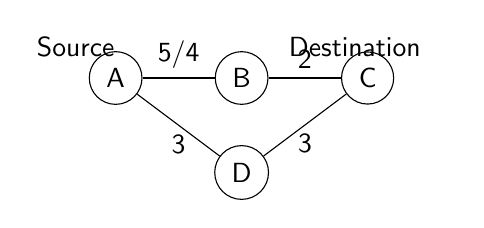
\begin{tikzpicture}[scale=0.8]
    \node[circle,draw] (A) at (0,0) {A};
    \node[circle,draw] (B) at (2,0) {B};
    \node[circle,draw] (C) at (4,0) {C};
    \node[circle,draw] (D) at (2,-1.5) {D};
    
    \draw (A) -- node[above] {5/4} (B);
    \draw (B) -- node[above] {2} (C);
    \draw (A) -- node[below] {3} (D);
    \draw (D) -- node[below] {3} (C);
    
    \node[text width=2cm] at (0,0.5) {Source};
    \node[text width=2cm] at (4,0.5) {Destination};
\end{tikzpicture}
\end{center}

\subsubsubsection{Classification of Routing Protocols}
\begin{itemize}
  \item \textbf{Proactive (Routing Table based):} when a packet needs to be forwarded, the \textcolor{red}{best route is already known (stored in the routing table)}
  \item \textbf{Reactive (Demand-based):} Determine the best route only when there is data to send
\end{itemize}

\subsubsubsection{Proactive Routing}
\begin{itemize}
  \item \textcolor{red}{Periodically} query for the possible routes in the network
  \begin{itemize}
    \item Save all routes that are important (maybe just all routes?)
    \item Also determine routes whenever topology changes (nodes join/leave)
  \end{itemize}
  \item \textbf{Upside:} when a packet arrives, route to destination is already known
  \item \textbf{Downside:} requires more memory and effort on part of routers
  \begin{itemize}
    \item Wastes some network bandwidth on checking for route changes
  \end{itemize}
\end{itemize}

\subsubsubsection{Reactive Routing}
\begin{itemize}
  \item Build up a map of the routes through a network
  \begin{itemize}
    \item Hopefully the ``optimal'' routes
  \end{itemize}
  \item Map routes in reaction to a packet arrival
  \begin{itemize}
    \item Sensor devices are slow and limited
    \item Most likely to resend to same prior address
    \item Discover a route when it is needed, then cache for next time
  \end{itemize}
\end{itemize}

\subsubsubsection{Ad-hoc Networks}
\begin{itemize}
  \item What if the nodes are not static but mobile?
  \item A Mobile Ad hoc Network (MANET) is an autonomous system of mobile nodes (MS) (also serving as routers) connected by wireless links
  \item No infrastructure exists in a MANET
  \item Network's wireless topology may change dynamically in an unpredictable manner since nodes are free to move, each node has limited transmitting power
  \item Assumption: Due to node mobility, routing path may be available but needs to be ``discovered''
\end{itemize}

\subsubsubsection{Ad-hoc On-demand Distance Vector Routing (AODV)}
\begin{itemize}
  \item \textbf{Ad-hoc:} dynamic and temporary networks
  \item \textbf{On-demand:} \textcolor{red}{Construct routes only when needed}
  \item \textbf{Distance vector:} routing metric is \textcolor{red}{the number of hops} a packet has to pass (\textcolor{red}{Hop Count})
\end{itemize}

\subsubsubsection{AODV Routing Table}
\begin{itemize}
  \item \textcolor{red}{Store the next hop} towards a destination, instead of storing a full path
  \begin{itemize}
    \item All routers along the path must also have Destination$\rightarrow$Next mappings
  \end{itemize}
  \item Also keep hops-to-destination and last-seen-destination-sequence-number
  \begin{itemize}
    \item Destination-sequence-number is an indicator of route freshness
  \end{itemize}
\end{itemize}

\subsubsubsection{AODV Route Discovery}
\begin{itemize}
  \item Upon demand: check table
  \item If not cached send \textcolor{red}{Route Request} (RREQ) via broadcasting
  \begin{itemize}
    \item Route is unknown, so broadcasting is needed
  \end{itemize}
\end{itemize}

\subsubsubsection{AODV Route Requests (RREQs)}
\begin{center}
  \begin{tabular}{|c|c|c|c|c|c|}
  \hline
  Request & Source & Destination & Source & Destination & \cellcolor{orange!60}Hop \\
  ID & Address & Address & SeqNo & SeqNo & \cellcolor{orange!60}Count \\
  \hline
  \end{tabular}
\end{center}

\begin{itemize}
  \item Request ID identifies this RREQ
  \begin{itemize}
    \item Used to discard duplicates during flooding
  \end{itemize}
  \item Sequence Numbers are per-device, monotonically increasing
  \begin{itemize}
    \item Used as a notion of ``how recently'' device has been seen
    \item Source SeqNo is the source's most recent sequence number
    \item Destination SeqNo is the most recently seen from the destination by the source (Defaults to zero)
  \end{itemize}
  \item Hop Count is the number of hops this request has taken
  \begin{itemize}
    \item Starts at 1 and incremented by each transmitter along the path
  \end{itemize}
\end{itemize}

\subsubsubsection{AODV Route Response (RREP)}
\begin{center}
  \begin{tabular}{|c|c|c|c|}
  \hline
  Source & Destination & Destination & \cellcolor{orange!60}Hop \\
  Address & Address & SeqNo & \cellcolor{orange!60}Count \\
  \hline
  \end{tabular}
\end{center}

\begin{itemize}
  \item Reply is sent unicast back to the source via newly constructed route
  \begin{itemize}
    \item Each node along the way already knows the route back
  \end{itemize}
  \item Includes recent destination sequence number as a sense of recency
  \begin{itemize}
    \item No need for source sequence number anymore
  \end{itemize}
\end{itemize}


\subsubsubsection{Route maintenance in AODV}
\begin{itemize}
  \item If a link in the routing table breaks, all active neighbors are informed with Route Error (RERR) messages
  \begin{itemize}
    \item After some number of retransmissions and timeouts
    \item RERR contains destination address that broke
  \end{itemize}
  \item Nodes receiving RERR can start RERQ for destination address
  \begin{itemize}
    \item Which lets them find a new path through the network
    \item And updates everyone's cached next-hops
  \end{itemize}
\end{itemize}

\subsubsubsection{Tradeoffs for reactive routing}
\begin{itemize}
  \item \textbf{Upside:} \textcolor{red}{no transmissions unless there is demand}
  \begin{itemize}
    \item Routes might appear, disappear, reappear, but no need to update if no one actually wants to transmit anything
  \end{itemize}
  \item \textbf{Downside:} large, \textcolor{red}{variable delay} when actually sending a packet
  \begin{itemize}
    \item Full RREQ/RREP protocol before data can actually be sent
    \item Route might have broken at some point
    \begin{itemize}
      \item So data will be sent based on cached information
      \item RERR will occur, RREQ/RREP will occur
      \item Then data will be sent again
    \end{itemize}
  \end{itemize}
\end{itemize}

\subsubsubsection{Load Balancing in Wireless Network}
% Add before Load Balancing section

\subsubsubsection{Many-to-one Sensor Networks}
\begin{itemize}
  \item \textcolor{red}{Data collection follows a spanning tree}
  \begin{itemize}
    \item All data is collected on a single node (gateway)
  \end{itemize}
  \item \textcolor{red}{Routing is simple:}
  \begin{itemize}
    \item Each device only needs to remember hop to gateway
    \item If gateway wants to send message back, it must include a full hop path
  \end{itemize}
  \item \textbf{Power consumption for each node}
  \begin{itemize}
    \item Per-node power consumption for data transmission and reception \textcolor{red}{grows exponentially} from the leaves to the root of the tree
    \item Power consumption increases at least linearly when nodes are closer to the sink
    \item Typical case is much worse
    \item Consequence: the power sources of the nodes close to the sink (gateway) deplete faster.
  \end{itemize}
\end{itemize}

\begin{center}
  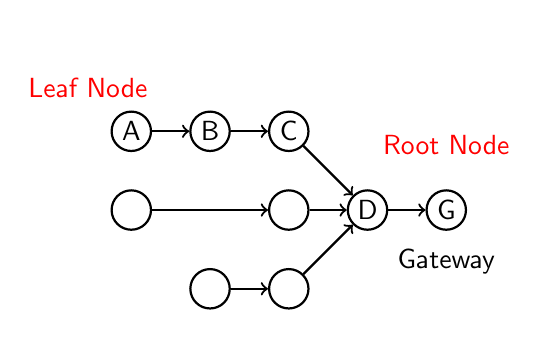
\begin{tikzpicture}[
    every node/.style={draw, circle, minimum size=5mm, inner sep=0mm},
    every path/.style={thick,->}
]

% Nodes
\node (A) at (0,3) {A};
\node (B) at (1,3) {B};
\node (C) at (2,3) {C};
\node (D) at (3,2) {D};
\node (G) at (4,2) {G};
\node (X1) at (0,2) {};
\node (X3) at (2,2) {};
\node (X2) at (1,1) {};
\node (X4) at (2,1) {};

% Edges
\draw (A) -- (B);
\draw (B) -- (C);
\draw (C) -- (D);
\draw (X1) -- (X3);
\draw (X3) -- (D);
\draw (D) -- (G);
\draw (X2) -- (X4);
\draw (X4) -- (D);
% Labels
\node[draw=none, above left, red] at (A) {Leaf Node};
\node[draw=none, above, red] at (G) {Root Node};
\node[draw=none, below, black] at (G) {Gateway};

\end{tikzpicture}
\end{center}


\subsubsubsection{In-network data aggregation}
\begin{itemize}
  \item To mitigate cost of forwarding, \textcolor{red}{compute relevant statistics along the way:} mean (A, B, C), max, min, median etc.
  \begin{itemize}
    \item E.g., Node C sends mean of (A, B, C)
    \item Send one value, instead of three separate messages
  \end{itemize}
  \item Forwarding nodes aggregate the data they receive with their own and send one message instead of relaying multiple messages
  \begin{itemize}
    \item Prevents exponentially growing number of messages
  \end{itemize}
  \item \textbf{Issues:}
  \begin{itemize}
    \item Location-based information is lost
    \item Distributed computation of statistics
    \begin{itemize}
      \item mean: node needs to know both the mean values and the sizes of samples to aggregate correctly
      \item median: only an approximated computation is possible
    \end{itemize}
  \end{itemize}
  \item \textbf{Applications:}
  \begin{itemize}
    \item Especially useful in a query-based data collection system
    \item Queries regard a known subset of nodes
    \item Aggregation function can be specified
  \end{itemize}
\end{itemize}

\subsection{Wifi}
\begin{itemize}
  \item Designed for high-speed communication over short indoor ranges
  \begin{itemize}
    \item Typical range: approximately 10 to 30 meters
    \item Primary use: connecting devices like laptops, mobile phones etc.
  \end{itemize}
\end{itemize}

\subsubsubsection{Basic WiFi network}
\begin{multicols}{2}
\begin{itemize}
  \item Star topology network
  \item A Basic Service Set includes:
  \begin{itemize}
    \item Access point(s) - AP
    \item Multiple connected clients
  \end{itemize}
  \item Service Set ID (SSID)
  \begin{itemize}
    \item Identifies network
    \item Broadcast by access point in beacons
  \end{itemize}
\end{itemize}
\end{multicols}


\subsubsubsection{Random Backoff in WiFi}
\begin{itemize}
  \item Carrier Sense Multiple Access
  \item Listen for activity
  \begin{itemize}
    \begin{multicols}{2}
      \item If free:
      \begin{itemize}
        \item Wait for Inter Frame Spacing (IFS)
        \item If still free, transmit
      \end{itemize}
      \item If busy:
      \begin{enumerate}
        \item Randomly select a number of backoff slots
        \item Count down slots whenever medium is not busy
        \item If busy when backoff completes:
        \begin{itemize}
          \item Increase maximum backoff slots
          \item Repeat
        \end{itemize}
      \end{enumerate}
    \end{multicols}

  \end{itemize}
  \item Slot time: basic time unit for protocol
  \begin{itemize}
    \item Total time of: switch from Rx to Tx, plus processing time, plus propagation delay
  \end{itemize}
\end{itemize}

\subsubsubsection{Prioritizing packets with varying IFS}
\begin{itemize}
  \item Tiered Contention Multiple Access (TCMA)
  \begin{itemize}
    \item Idea: assign different inter-frame spacing based on traffic class
    \item Inherently prioritizes communication
  \end{itemize}
  \item Acknowledgements sent with Short IFS (SIFS)
  \begin{itemize}
    \item Will always transmit before new data clears CSMA check
  \end{itemize}
  \item Regular data sent with DIFS
  \item SIFS < PIFS < DIFS
\end{itemize}

\includegraphics*[width=8.5cm, height=2cm]{images/ifs.png}

\subsubsubsection{FHSS}
\begin{itemize}
  \item Frequency Hopping Spread Spectrum
  \item Frequency hopping over 80 channels (1 MHz each)
  \item Have the transmitter hop between a seemingly random sequence of frequencies
  \item Spreading pattern shared by pairs of sender and receiver
  \item FHSS is one type of \textit{Spread Spectrum technique}
\end{itemize}

\begin{center}
\includegraphics*[width=8.5cm, height=2.5cm]{images/fhss.png}
\end{center}

\subsubsubsection{Direct Sequence Spread Spectrum (DSSS)}
\begin{itemize}
  \item Each bit of information is coded so that it uses a larger bandwidth
  \item Essentially, each bit is \textcolor{red}{multiplied by a sequence of bits} with a much higher data rate
\end{itemize}

\begin{center}
  \includegraphics*[width=8.5cm, height=2.5cm]{images/dsss.png}
  \includegraphics*[width=8.5cm, height=4cm]{images/dsss2.png}
\end{center}

\subsubsubsection{DSSS properties}
\begin{itemize}
  \item DSSS increases bandwidth of a signal
  \begin{itemize}
    \item Beyond what is needed for the data
    \item Energy is smeared across the frequencies
  \end{itemize}
  \item More robust against interference
  \begin{itemize}
    \item Data can be recovered from partial code
  \end{itemize}
  \item \textcolor{red}{Data Rate better than FHSS}
  \begin{itemize}
    \item DSSS transmits continuously over a wide band
    \item FHSS has to switch frequencies, introducing delays during each hop
  \end{itemize}
  \item Cost: using a lot of bandwidth for only a little data
  \item GPS uses DSSS
\end{itemize}

\subsubsubsection{Spread Spectrum Summary}
\begin{itemize}
  \item Spreading out the signals over a wide channel
  \begin{itemize}
    \item FHSS (multi-frequency hops)
    \item DSSS (single frequency)
  \end{itemize}
  \item Spread Spectrum:
  \begin{itemize}
    \item Add Redundancy in frequency domain
    \item \textcolor{red}{Spread transmission much wider spectrum band} than needed for the intended bit rate
    \item Key idea: traffic of other users looks like noise
  \end{itemize}
  \item Cellular 3G (CDMA) builds on spread spectrum
  \begin{itemize}
    \item Each pair of the TX and RX must coordinate so RX can apply the same code to decode the data
  \end{itemize}
\end{itemize}

\subsubsubsection{OFDM}
\begin{itemize}
  \item \textbf{OFDM:} \textcolor{teal}{orthogonal} \textcolor{red}{frequency division multiplexing}
  \item \textbf{Channel Impact - Multipath:}
  \begin{itemize}
    \item \textbf{Key Issues:}
    \begin{itemize}
      \item Frequency selective fading: Induces significant impact at \textcolor{red}{high data rates} and on \textcolor{red}{wide-band channels}
      \item Inter-symbol interference (ISI): As rates increase, symbol duration shrinks, making ISI effects more pronounced
    \end{itemize}
    \item Caused by signal reflection from objects (e.g., walls) creating multiple paths
    \item \textbf{Solution needed:} An encoding/modulation solution to mitigate multipath effect
  \end{itemize}
\end{itemize}

\includegraphics*[width=8.5cm, height=4.5cm]{images/intersymbolinterference.png}

\subsubsubsection{Key Idea | Frrequency Division Multiplexing}
\includegraphics*[width=8.5cm, height=4cm]{images/distributebitsoversubcarriers.png}

\begin{itemize}
  \item Each subcarrier is a narrow-band signal with a different center frequency
  \item Symbol duration \textcolor{red}{increases} with number of carriers, more resistance to ISI
  \item \textbf{Implementation:}
  \begin{itemize}
    \item \textcolor{red}{Distribute bits over N subcarriers} that use different frequencies over the band with \textcolor{red}{B bandwidth}
    \item Each signal uses $\sim$ B/N bandwidth
    \item Multi-carrier modulation
  \end{itemize}
  \item \textbf{Benefits:}
  \begin{itemize}
    \item Since each subcarrier only encodes 1/N of the bit stream, each symbol can \textcolor{red}{take N times longer in time}
    \item Since \textcolor{red}{signals are narrower} in spectrum, frequency-selective fading is mitigated
  \end{itemize}
\end{itemize}

\includegraphics*[width=8.5cm, height=4cm]{images/fdmillustration.png}

\subsubsubsection{Why Orthogonal in OFDM}
\includegraphics*[width=8.5cm, height=4cm]{images/ofdmillustration.png}
\begin{itemize}
  \item \textbf{Goal:} \textcolor{teal}{To achieve even higher data rate}
  \item \textbf{Challenge:} How to pack multiple subcarriers very densely?
  \begin{itemize}
    \item Need to support 48 or more subcarriers
    \item Must avoid interference between subcarriers
    \item Traditional FDM uses guard bands between adjacent subcarriers
  \end{itemize}
  \item \textbf{Solution:} Orthogonal subcarriers
  \begin{itemize}
    \item Allows denser packing of subcarriers without interference
    \item More efficient use of available bandwidth compared to traditional FDM
  \end{itemize}
\end{itemize}

\subsubsubsection{Orthogonal Subcarriers}
\includegraphics*[width=8.5cm, height=2.5cm]{images/orthogonalsubcarriers.png}
\begin{itemize}
  \item Peaks of spectral density of each carrier falls exactly at the zeros of the other carriers
  \item Carriers can be packed densely with minimal interference
\end{itemize}

\subsubsubsection{OFDM enables higher throughput}
\begin{itemize}
  \item \textbf{Evolution:} Replace DSSS with Orthogonal Frequency Division Multiplexing
  \item \textbf{OFDM Approach:}
  \begin{itemize}
    \item Split band into a number of narrow subcarriers
    \item Subcarriers are spaced so that they don't interfere
    \item Transmit on multiple subcarriers at once to increase throughput
  \end{itemize}
  \item \textbf{Implementation:}
  \begin{itemize}
    \item Receivers collect signal from entire channel
    \item Can split it apart to gain data on each subcarrier
    \item Process: Frequency-Domain QAM → IFFT → Time-Domain Signal → FFT → Recovered QAM Data
  \end{itemize}
  \item \textbf{Advantages:}
  \begin{itemize}
    \item Higher spectral efficiency through dense subcarrier packing
    \item Parallel transmission across multiple subcarriers
    \item Better handling of multipath effects
  \end{itemize}
  \item \textbf{Tradeoffs:}
  \begin{itemize}
    \item Benefits: more throughput, still robust against narrowband interference
    \item Costs: more complicated and sensitive radio design
  \end{itemize}
\end{itemize}

\subsubsubsection{802.11a - First WiFi with OFDM}
\begin{itemize}
  \item \textbf{Implementation (1999):}
  \begin{itemize}
    \item Applied OFDM techniques on the \textcolor{red}{5 GHz band}
    \item Enabled more data throughput \textcolor{red}{54 Mbps} (compare to 11 Mbps for 802.11b)
  \end{itemize}
  \item \textbf{Multiple rates available:}
  \begin{itemize}
    \item BPSK/QPSK/QAM over OFDM
    \item Quadrature Amplitude Modulation (QAM)
  \end{itemize}
  \item \textbf{Channel Structure:}
  \begin{itemize}
    \item Several 20 MHz channels with no overlap
    \item Big increase from "three" channels of 2.4 GHz
    \item Various regional rules on number of different channels
    \item Needs to avoid frequencies in use by existing radar deployments
  \end{itemize}
  \item Never reached widespread adoption
  \begin{itemize}
    \item Regulatory hurdles in some regions
    \item More complicated hardware delayed it
  \end{itemize}
\end{itemize}


\subsubsubsection{Use multiple antennas to increase throughput}
\includegraphics*[width=8.5cm, height=2.2cm]{images/multiantennas.png}
\begin{itemize}
  \item \textbf{Multiple Antenna Benefits:}
  \begin{itemize}
    \item \textcolor{red}{Receive multiple copies} of the same signal
    \item \textcolor{red}{Combine copies to improve signal quality} (e.g., stronger, clearer)
    \item More robust performance in noisy environments
    \item Better signal \textcolor{red}{allows for faster data transmission}
    \begin{itemize}
      \item Enables higher data rates without extra bandwidth
    \end{itemize}
  \end{itemize}
  \item \textbf{Multiple Antenna Configurations:}
  \begin{itemize}
    \item Multiple transmitters to single receiver (2$\rightarrow$1)
    \item Single transmitter to multiple receivers (1$\rightarrow$2)
    \item Each configuration provides different benefits for signal quality and reliability
  \end{itemize}
\end{itemize}

\subsubsubsection{MIMO - Multiple Input Multiple Output}
\begin{itemize}
  \item \textbf{Architecture:}
  \begin{itemize}
    \item N transmit antennas communicate with M receive antennas
    \item Creates $N \times M$ subchannels for simultaneous data transmission
  \end{itemize}
  \item \textbf{Benefits:}
  \begin{itemize}
    \item \textcolor{red}{Huge boost in data throughput}
    \item Antenna diversity adds to \textcolor{red}{reliability} as well
  \end{itemize}
  \item \textbf{Signal Processing:}
  \begin{itemize}
    \item The signals may interfere with each other
    \item But receiving all of them allows the data to be recovered
  \end{itemize}
  \item \textbf{Beamforming:}
  \begin{itemize}
    \item Use interactions between array of antennas to focus energy on the receiver
  \end{itemize}
\end{itemize}

\subsubsubsection{802.11n - Wider channels and MIMO}
\begin{itemize}
  \item \textbf{Channel Width (2009):}
  \begin{itemize}
    \item OFDM allows many subcarriers within a channel to be used at once
    \item Throughput scales with the amount of bandwidth available
    \item Allow larger \textcolor{red}{40 MHz channels} to be used
  \end{itemize}
  \item \textbf{Dual-band Support:}
  \begin{itemize}
    \item Supports OFDM and MIMO on 2.4 GHz and 5 GHz
    \item Supports 20 MHz and 40 MHz channels
    \item Easier to create large channels in 5 GHz band
  \end{itemize}
  \item \textbf{Compatibility:}
  \begin{itemize}
    \item Backwards compatible with 802.11g (tries not to be with 802.11b)
    \item Wildly successful
    \begin{itemize}
      \item Still the 2.4 GHz band protocol (802.11ac is 5 GHz only)
      \item A little less than half of the networks visible are still 802.11n
    \end{itemize}
  \end{itemize}
\end{itemize}

\includegraphics*[width=8.5cm, height=4.2cm]{images/multimimo.png}
\subsubsubsection{802.11ac - Enhanced MIMO and wider channels}
\begin{itemize}
  \item \textbf{Implementation (2013):}
  \begin{itemize}
    \item Update for \textcolor{red}{5 GHz band only}
    \item Supports Downlink MU-MIMO (from AP to device)
    \item Supports channel widths up to \textcolor{red}{160 MHz}
    \item Engineering updates: up to 256-QAM
  \end{itemize}
  \item \textbf{Deployment Strategy:}
  \begin{itemize}
    \item \textcolor{red}{Routers apply 802.11ac to 5 GHz and 802.11n to 2.4 GHz}
  \end{itemize}
\end{itemize}

\subsubsubsection{WiFi 6 - Focus on Network Efficiency}
\begin{itemize}
  \item \textbf{Primary Goal:} Improve \textcolor{red}{total throughput} across all devices in the network
  \item \textbf{Context:}
  \begin{itemize}
    \item For point-to-point, WiFi is "(more than) fast enough"
    \item Now the problem is the quantity of devices in a single space
    \begin{itemize}
      \item Desktop, laptop, tablet, smartphone, smartwatch, IoT devices, etc.
    \end{itemize}
  \end{itemize}
  \item \textbf{Solution Approach:}
  \begin{itemize}
    \item Insight: Bring established cellular techniques to WiFi
    \item Focus on managing multiple concurrent connections efficiently
  \end{itemize}
\end{itemize}

\subsubsubsection{OFDMA - Efficient Multi-user Access}
\includegraphics*[width=8.5cm, height=2.2cm]{images/ofdma.png}
\begin{itemize}
  \item \textbf{OFDM vs OFDMA:}
  \begin{itemize}
    \item OFDM: split channel into subcarriers and transmit on those
    \item OFDMA: \textcolor{red}{allocate subcarriers to a device for an amount of time}
  \end{itemize}
  \item \textbf{Key Innovation:}
  \begin{itemize}
    \item Turns OFDM into an \textcolor{red}{access control mechanism}
    \item Complicated question: which device gets which subcarriers at which time?
  \end{itemize}
  \item \textbf{Benefits:}
  \begin{itemize}
    \item More efficient use of available bandwidth
    \item Multiple users can transmit simultaneously
    \item Reduced latency for small data transfers
  \end{itemize}
\end{itemize}

\subsubsubsection{802.11ax (WiFi 6) - 6 GHz Band Extension}
\begin{itemize}
  \item \textbf{Standard Timeline:}
  \begin{itemize}
    \item Standard approved on February 9\textsuperscript{th} 2021
    \item First devices started supporting it in 2019 (WiFi 6)
  \end{itemize}
  \item \textbf{6 GHz Band (WiFi 6E):}
  \begin{itemize}
    \item \textcolor{red}{1.2 GHz of bandwidth} (5.925-7.125 GHz)
    \item 2020: US FCC made band available for unlicensed use
    \item EU followed in March 2021
  \end{itemize}
  \item \textbf{OFDMA Implementation:}
  \begin{itemize}
    \item MAC scheduling variant of OFDM
    \item Schedule devices based on time and subcarrier allocations
  \end{itemize}
\end{itemize}

\end{multicols*}




\begin{tabular}{|p{2.5cm}|p{3.5cm}|p{3.5cm}|p{3.5cm}|}
  \hline
  \rowcolor[gray]{0.8}
  \textbf{Feature} & \textbf{FDMA} & \textbf{TDMA} & \textbf{OFDM} \\
  \hline
  Channel Access & Divides channel into frequency bands, each user assigned a specific frequency & Divides channel into time slots, each user assigned a specific time slot & Uses multiple orthogonal subcarriers simultaneously \\
  \hline
  Collision Handling & No collisions within allocated frequency bands & No collisions within allocated time slots & Minimizes collisions through orthogonal frequency division \\
  \hline
  Efficiency & Medium: Bandwidth may be wasted if user has no data to send & Medium-High: Time slots may be wasted if user has no data to send & High: Efficient spectrum usage through parallel transmissions \\
  \hline
  Interference & Vulnerable to narrowband interference & Less vulnerable to frequency-specific interference & Resistant to narrowband interference and multipath fading \\
  \hline
  Synchronization & No tight synchronization needed & Requires precise time synchronization & Requires frequency synchronization \\
  \hline
  Best Used In & Simple constant-bit-rate applications, analog systems & Digital cellular systems, satellite communications & Modern wireless networks (Wi-Fi, 4G/5G), high-speed data transmission \\
  \hline
  \end{tabular}

  
  \begin{tabular}{|p{2.5cm}|p{3.5cm}|p{3.5cm}|p{3.5cm}|}
  \hline
  \rowcolor[gray]{0.8}
  \textbf{Feature} & \textbf{Aloha} & \textbf{Slotted Aloha} & \textbf{CSMA} \\
  \hline
  Channel Access & Transmits immediately when data is ready without checking channel status & Transmits only at beginning of predetermined time slots & Listens to the channel before transmitting (sense-before-send) \\
  \hline
  Collision Handling & Collisions occur frequently due to uncoordinated transmissions & Reduced collisions compared to pure Aloha, but still occur & Significantly reduces collisions by avoiding transmission when channel is busy \\
  \hline
  Retransmission & Random backoff time before retrying after collision & Random waiting time before retrying, synchronized to slots & Uses various backoff algorithms (e.g., exponential) to reduce subsequent collisions \\
  \hline
  Efficiency & Very low: ~18\% of channel capacity & Low-Medium: ~36\% of channel capacity & Medium-High: Up to 80\% in optimal conditions \\
  \hline
  Collision Avoidance & None; simply retransmits after collision & None; retransmits at next available slot & Various mechanisms like RTS/CTS and collision detection depending on variant \\
  \hline
  Best Used In & Simple, very low-traffic networks & Networks with predictable traffic patterns & Wireless and wired LANs with variable traffic loads \\
  \hline
  \end{tabular}

  
  \begin{tabular}{|p{2.5cm}|p{3.5cm}|p{3.5cm}|p{3.5cm}|}
  \hline
  \rowcolor[gray]{0.8}
  \textbf{Feature} & \textbf{ALOHA with preamble} & \textbf{B-MAC} & \textbf{X-MAC} \\
  \hline
  Channel Access & Sends a preamble before data transmission to announce intent & Uses Low Power Listening (LPL) with long preambles & Uses shortened preambles with target address \\
  \hline
  Collision Handling & Reduced collisions compared to pure Aloha & Collisions reduced through channel sensing & Improved collision avoidance through early acknowledgment \\
  \hline
  Power Efficiency & Low: Continuous listening & Medium: Periodic channel sampling & High: Early acknowledgment reduces overhearing \\
  \hline
  Latency & Medium & High due to long preamble & Reduced compared to B-MAC \\
  \hline
  Adaptability & Limited adaptability to traffic patterns & Configurable sleep intervals & Adaptable to varying traffic patterns \\
  \hline
  Best Used In & Simple networks with low power constraints & Wireless sensor networks with low duty cycles & Energy-constrained sensor networks with variable traffic \\
  \hline
  \end{tabular}

\end{document}
